\documentclass[10pt,a4paper]{report}
\usepackage{german,url}
\usepackage{color}
\usepackage{times}
\usepackage{amssymb}
\usepackage{amsmath}
\usepackage{verbatim}
\usepackage{vmargin}
\usepackage{t1enc}
\usepackage[T1]{fontenc}
\usepackage[german]{babel}
\usepackage[latin1]{inputenc}
\usepackage[pdftex]{graphicx}
\usepackage[pdftex]{graphics}
\usepackage[pdfborder=0]{hyperref}
\author{Hauke Goos-Habermann\\ mit Ausz�gen des alten Handbuches von Ralf S�rensen}
\title{m23-Benutzerhandbuch\\
\includegraphics{/mdk/doc/manual/screenshots/m23biglogo.jpg}\\m23 rock 13.2
}

\begin{document}
\maketitle

\tableofcontents

Welcome to the m23 development guide. This is a not (yet) finished document because m23 isn't completed yet. You will find useful information about the m23 interna. If you want to develop for m23 this is the right document for you ;).\\
If you don't know what m23 is, you'll get a short answer. m23 will help you to set up hundreds of clients from one place. m23 can partition and format clients, install an operating system and additional programs. With m23 you can manage your clients and keep them up to date. For more information have a look at the m23 user guide.\\
This guide is meant for developers and people who want to know how m23 works only.
\section{What you can expect from this document:}
\begin{itemize}
\item an API reference about all functions used in the m23admin GUI and packages. This will be useful if you want to make changes to m23, build addons or plugins.
\item information about serveral tools developed for m23. The little tools called "m23 helpers" make m23 work. Without them m23 can't do its job. You will learn how these tools work and how to use them.
\end{itemize}
\section{What you can't exspect from this document:}
\begin{itemize}
\item a 100\% description of all functionality of m23. m23 is still in development, things are changing rapidly, so don't expect too much actuality.
\item correct english ;) But I think it is written in a way most people will be able to understand. Don't expect a poem ;)
\end{itemize}
Have fun ;)

\chapter{Requirements for m23}
If you want to integrate the software distribution system m23 into your network you need the following components:
\begin{itemize}
\item m23 server
\item m23 client(s)
\item Internet access
\item PC with webbrowser
\item m23 server installation CD
\end{itemize}

\section{The m23 server}
The m23 server performs the complete software distribution and fulfils different tasks:
\begin{itemize}
\item Generation of the web interface
\item Compilation of installation scripts "on-the-fly"
\item Software package cache
\item Database
\item Boot server
\item DHCP server
\end{itemize}
You should dimension your m23 server with enough RAM and an adequate processor. If you want to use the server only for a few clients or for testing purpose you can try it with an older computer (e.g. P1 with 166MHz and 64MB RAM). For bigger networks the server should not have less than 256MB RAM. In all cases the server needs a network card and a harddisk with 5 or more GB of free space. If you want to install a big variety of software packages on your clients you need a harddisk with a lot of space to make caching of these packages possible.
\begin{itemize}
\item CPU: from 166Mhz up (recommended  1GHz)
\item RAM: from 64MB up (recommended  from 256MB)
\item Harddisk: from 5GB up
\item Network card: recommended 100MBit/1GBit
\end{itemize}

\section{The m23 clients}
For clients the recommendations are roughly the same. To facilitate software distribution for you, you should use wake-on-lan-able clients which can be started for installation and shutdowned afterwards by m23. It is a good idea to use network cards containing a bootrom to allow the clients to be installed without using a boot disk or a CD. They will be necessary for the installation of the operating system only. m23 supports PXE and Etherboot boot standards.

\section{Internet access}
m23 needs access to the internet to fetch the software packages that can be installed on the clients.

\section{PC with webbrowser}
For your administration you need a PC with a web browser to access the m23 server.

\section{The server installation CD}
To install the m23 server you need the m23 server installation CD which can be downloaded for free from  \underline{http://m23.sf.net}. Burn the ISO file on a CD and boot the server from it.
\chapter{Installation du serveur}
\section{Pr�parations}
Avant que vous commenciez avec l'installation de votre serveur m23, vous devriez faire quelques consid�rations:
\begin{itemize}
\item Est-ce que mon serveur et les clients accordent les exigences (regardez le chapitre pr�c�dent)?
\item Comment est-ce que mon r�seau est organis�?
\item Quel num�ro IP est-ce que je veux assigner au serveur?
\item Quels sont les ajustements pour le masque du r�seau, la passerelle, le serveur de noms de domaine et le num�ro IP du r�seau?
\item Est-ce que le lecteur CD-ROM de mon serveur est capable d'amorcer?
\end{itemize}

\section{Commencer avec l'installation}
Connectez le serveur au r�seau et inserez le CD de l'installation de m23 dans le lecteur. Tenez les ajustements de r�seau n�cessaires � main. L'installation s'explique de soi et ne devrait pas poser des probl�mes � quelqu'un qui a des connaissance des concepts fondamentals de l'administration d'un r�seau. Au suivant, vous verrez des copies d'�cran de l'installation, que le serveur va parcourir. Ne vous inqui�tez pas quand il y a encore d'autres affichages sur votre moniteur pendant la procedure de l'installation - je ne le croyais pas utile de d�montrer toutes affichages d'�tat en des copies d'�cran  ;).\\\\

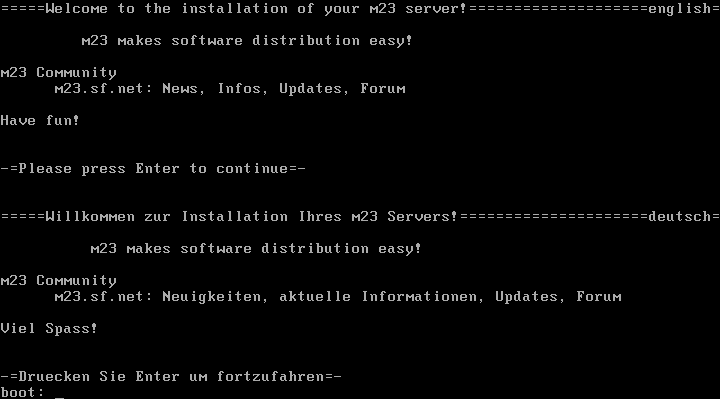
\includegraphics[scale=0.45]{/mdk/doc/manual/screenshots/serverinstall/en/inst1.png}\\
Ceci est l'affichage d'amor\c{c}age du CD de l'installation de m23. Apr�s que vous ayez appuy� sur la touche Retour, le syst�me d'exploitation Linux amorcera du CD et commencera avec le programme de l'installation.


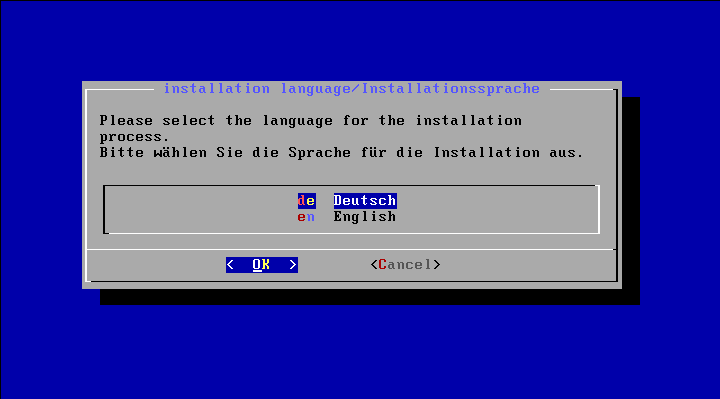
\includegraphics[scale=0.45]{/mdk/doc/manual/screenshots/serverinstall/en/inst2.png}\\
Vous pouvez choisir si vous voulez ex�cuter le programme d'installation en allemand ou en anglais. Ici, nous supposons que vous vous d�ciderez pour l'anglais. 

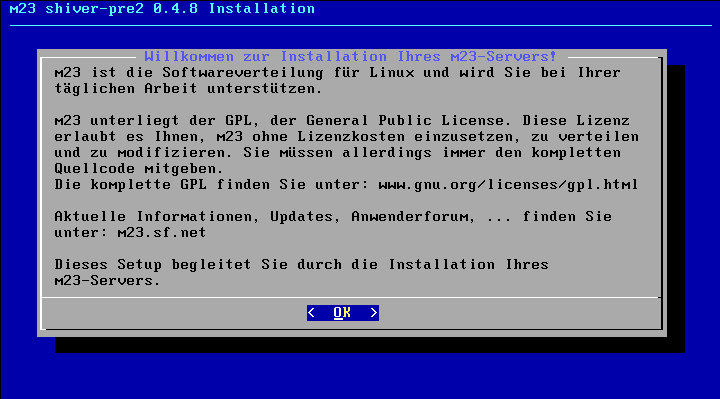
\includegraphics[scale=0.45]{/mdk/doc/manual/screenshots/serverinstall/en/inst3.png}\\
Un petit $\ll$Bienvenu$\gg$.



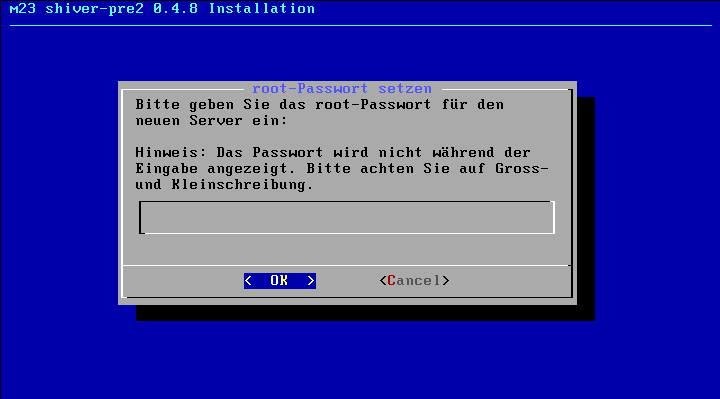
\includegraphics[scale=0.45]{/mdk/doc/manual/screenshots/serverinstall/en/inst4.png}\\
Entrez le mot de passe de la racine. Root (racine) est l'administrateur du syst�me avec acc�s illimit� au serveur m23. Vous devriez choisir un mot de passe qui ne peut pas �tre devin� facilement et qui consiste au moins de 10 caract�res. Vous devriez aussi employer des caract�res sp�ciaux, des chiffres et des majuscules et des minuscules.\\
Comme le mot de passe n'est pas montr�e, il sera control� par une deuxi�me entr�e dans le dialogue suivant.



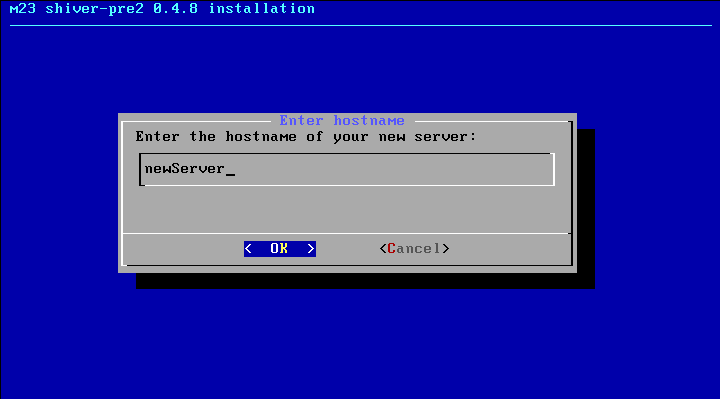
\includegraphics[scale=0.45]{/mdk/doc/manual/screenshots/serverinstall/en/inst5.png}\\
Le $\ll$hostname$\gg$ est le nom pour le serveur.



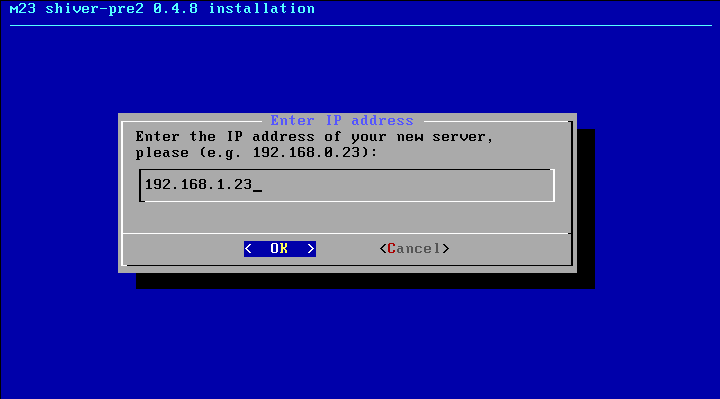
\includegraphics[scale=0.45]{/mdk/doc/manual/screenshots/serverinstall/en/inst6.png}
\\
L'adresse IP que vous voulez assigner au serveur. Vous devriez choisir l'adresse d'une fa\c{c}on qui rend les clients capable d'atteindre le serveur sans l'emploi d'un routeur.


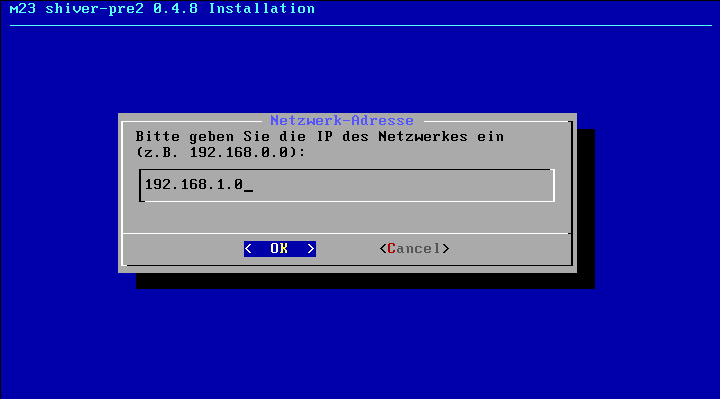
\includegraphics[scale=0.45]{/mdk/doc/manual/screenshots/serverinstall/en/inst7.png}\\
L'adresse du r�seau. C'est l'adresse sous laquelle le r�seau est accessible.



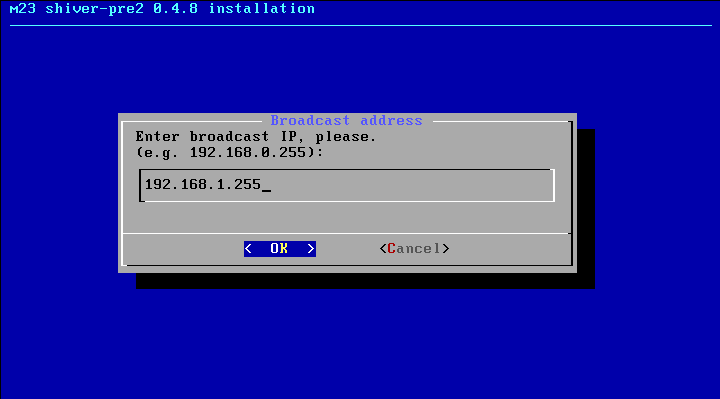
\includegraphics[scale=0.45]{/mdk/doc/manual/screenshots/serverinstall/en/inst8.png}
\\



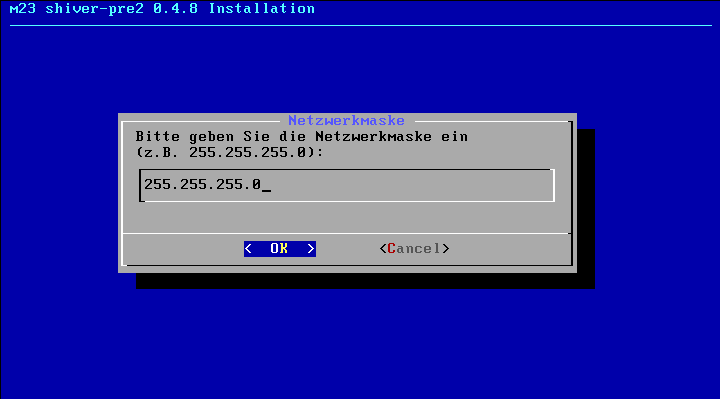
\includegraphics[scale=0.45]{/mdk/doc/manual/screenshots/serverinstall/en/inst9.png}
\\
Le masque du r�seau indique, quelle partie de l'adresse IP appartient au ordinateur particulier et quelle partie masque le r�seau.



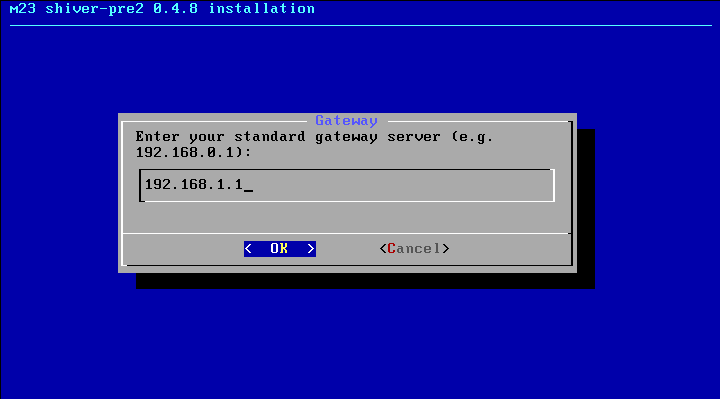
\includegraphics[scale=0.45]{/mdk/doc/manual/screenshots/serverinstall/en/inst10.png}
\\
L'IP de la passerelle indique l'adresse IP, par laquelle les demandes aux adresses IP sont dirig�es, qui se trouvent hors du r�seau du serveur.



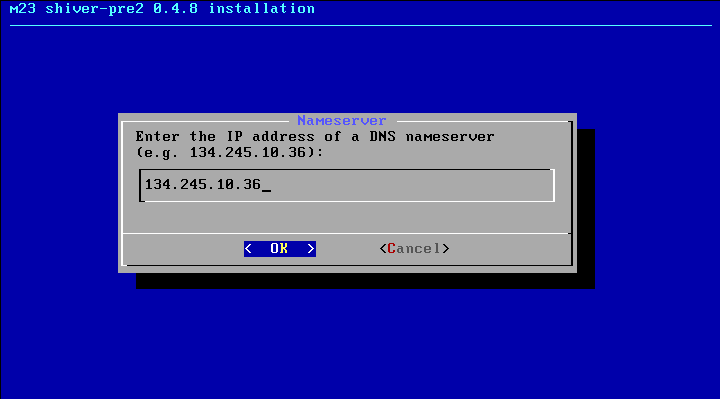
\includegraphics[scale=0.45]{/mdk/doc/manual/screenshots/serverinstall/en/inst11.png}
\\
Pour la dissolution des noms URL en des adresses IP, il est n�cessaire d'employer un serveur de noms DNS, qui ex�cute la transformation. Par exemple, ftp.debian.org devient 128.101.80.131. Si vous ne connaissez pas de serveur de noms DNS, vous pouvez utiliser l'adresse IP 134.245.10.36. Celle-ci est l'adresse du serveur de noms DNS de l'universit� de Kiel.



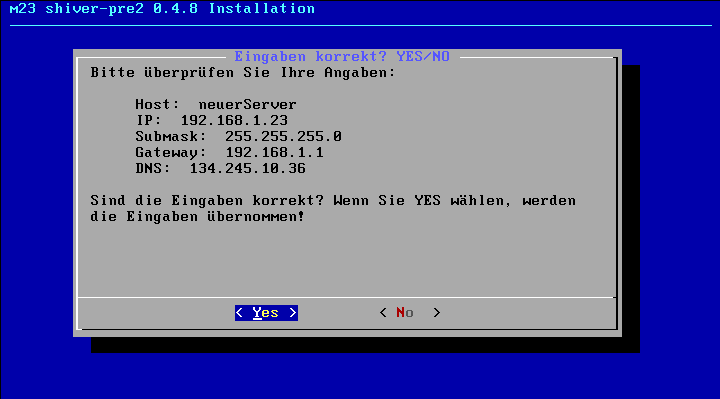
\includegraphics[scale=0.45]{/mdk/doc/manual/screenshots/serverinstall/en/inst12.png}
\\
Ici, vous avez la possibilit� de contr\^oler, si vos entr�es sont correctes. Si vous voulez continuer avec l'installation, choisissez $\ll$Yes$\gg$, sinon, vous pouvez corriger vos entr�es apr�s avoir choisi $\ll$No$\gg$.

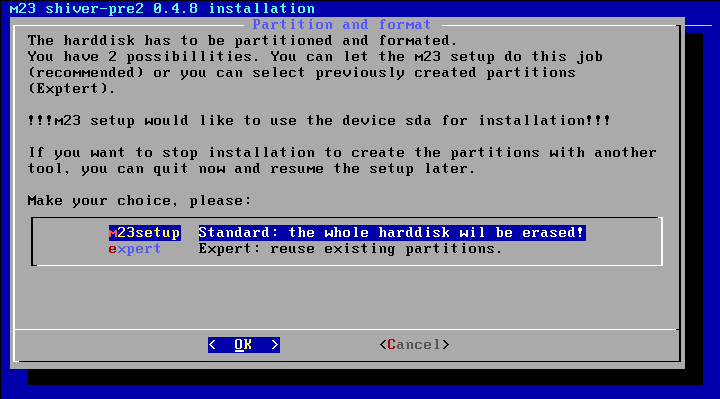
\includegraphics[scale=0.45]{/mdk/doc/manual/screenshots/serverinstall/en/inst13.png}
\\
Ici, vous pouvez choisir si vous voulez employer le disque dur tout entier du serveur pour m23. Cela a pour r�sultat que 2 partitions seront �tablies, une pour le syst�me d'exploitation Debian/Linux et une pour la permutation. S'il y a plusieurs disques durs, le premier sera utilis�. Mais vous pouvez aussi utiliser des partitions que vous avez �tablies auparavant si vous souhaitez un partitionnement sp�cial.\\\\
\underline{Information suppl�mentaire concernant le partitionnement}
Notez que, pendant l'installation, le serveur sera effac� compl�tement si vous n'avez pas �tabli deux partitions sur le premier disque dur (hda ou sda) avec un programme comme Parted, fdisk, cfdisk etc. comme c'est indiqu� au suivant:
\begin{itemize}
\item une partition pour m23 d'une taille de 4 GB au moins
\item une partition pour la permutation pour Linux (recommand� d'une taille deux fois la taille de la m�moire vive)
\end{itemize}
Notez les adresses des partitions, s.v.p. Par exemple la premi�re partition du premier disque dur est nomm�e hda1 et la deuxi�me hada2. Si vous utilisez une partition �tendue, la premi�re partition dans la partition �tendue sera nomm�e hda5, la deuxi�me hda6 etc. Vous serez demand� ces adresses pendant l'installation, si vous avez choisi le type $\ll$experte$\gg$ pour le partitionnement.
Nous recommandons � la plupart des utilisateurs de sauvegarder les donn�es et de laisser m23 partitionner et formater le serveur entier.


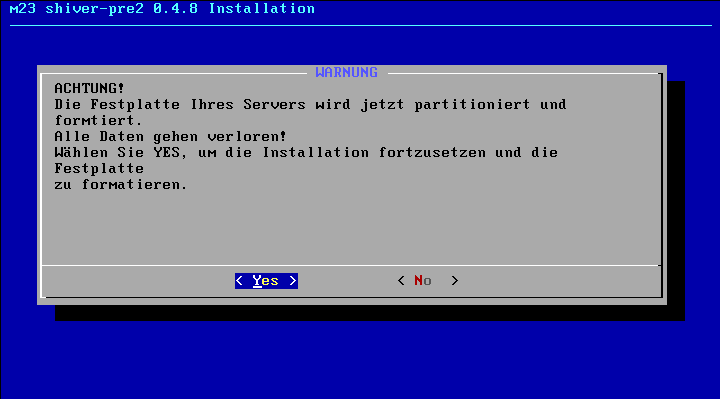
\includegraphics[scale=0.45]{/mdk/doc/manual/screenshots/serverinstall/en/inst14.png}
\\
Le dernier avertissement ;)



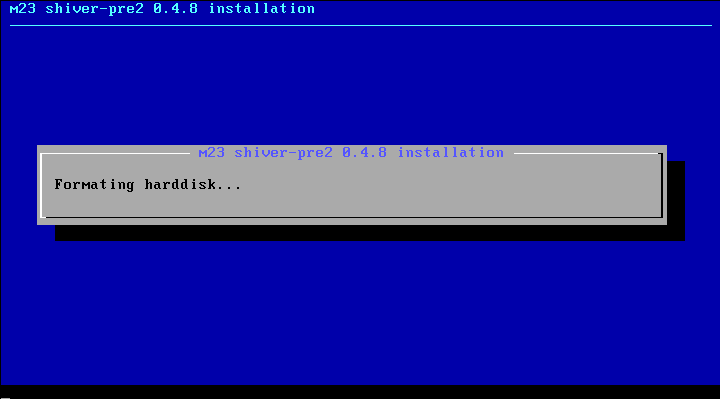
\includegraphics[scale=0.45]{/mdk/doc/manual/screenshots/serverinstall/en/inst15.png}
\\



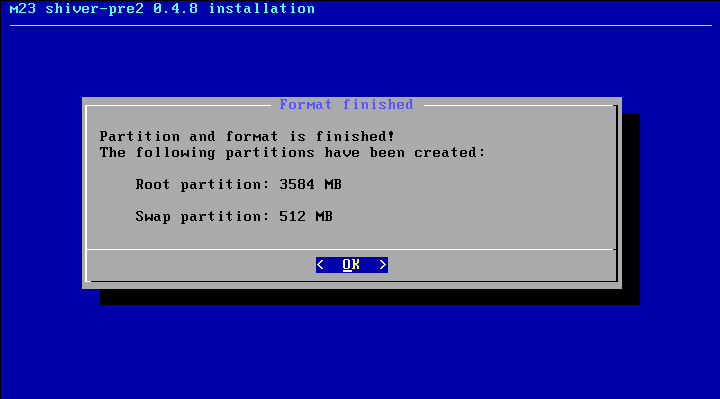
\includegraphics[scale=0.45]{/mdk/doc/manual/screenshots/serverinstall/en/inst16.png}
\\



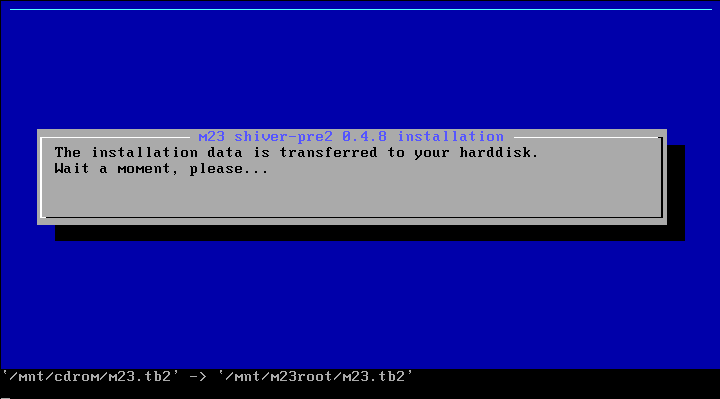
\includegraphics[scale=0.45]{/mdk/doc/manual/screenshots/serverinstall/en/inst17.png}
\\


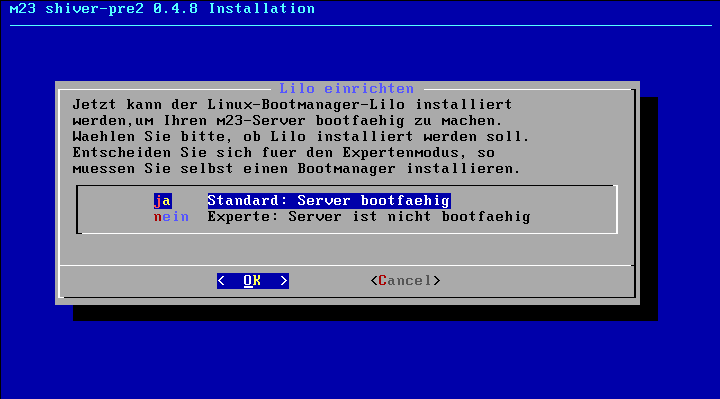
\includegraphics[scale=0.45]{/mdk/doc/manual/screenshots/serverinstall/en/inst18.png}
\\
Ici, vous pouvez d�cider si vous voulez installer le gestionnaire d'amor\c{c}age LILO (LInux LOader). Ceci sera install� dans le MBR (MasterBootRecord) du premier disque dur. Si vous vous d�cidez contre, vous devez installer un gestionnaire d'amor\c{c}age vous-m�me. Sinon, le serveur m23 ne peut pas amorcer.


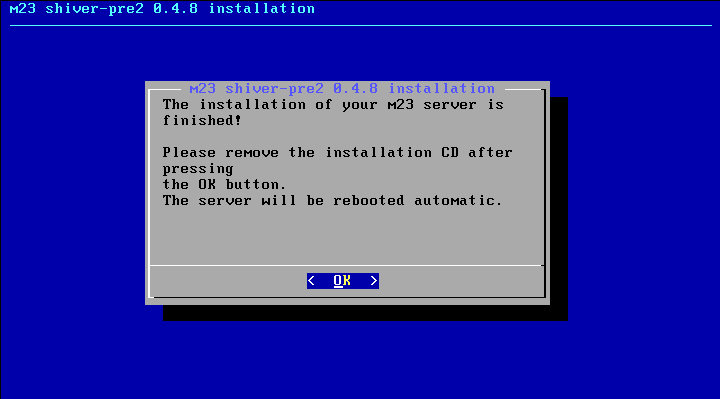
\includegraphics[scale=0.45]{/mdk/doc/manual/screenshots/serverinstall/en/inst19.png}
\\
L'installation est termin�e ;)
\section{Fin de l'installation}
\underline{Notez}: Vous n'avez pas besoin d'un moniteur en service normal, except� que vous le voulez utiliser aussi pour le travail. Comme le serveur m23 est bas�e sur un syst�me Debian GNU/Linux, vous pouvez ouvrir un session comme root comme d'habitude et installer du logiciel additionel comme c'est l'usage avec Debian. Regardez \underline{www.debian.org} pour des informations suppl�mentaires.\\
Maintenant, vous pouvez ajouter votre premier client!

\chapter{Erste Schritte mit dem m23-Server}
\section{Verbindung zum m23-Server aufnehmen}
Nachdem Sie Ihren Server erfolgreich installiert und neu gestartet haben, gelangen Sie �ber einen beliebigen Webbrowser auf einem am Netzwerk angeschlossenen PC auf die m23-Administrationsoberfl�che. Geben Sie dazu in Ihrem Webbrowser folgende Ziel-URL ein:\\\\
\underline{http://ServerIP}\\\\

Als ServerIP nehmen Sie bitte die IP Ihres m23-Servers (z.B.: 192.168.1.23). Beim ersten Einloggen haben Sie noch kein eigenes m23-Administrator-Konto, deshalb geben Sie bitte das LOGIN und PASSWORT ein, welches auf der Hintergrundfl�che steht. Sobald Sie eingeloggt sind, sollten Sie sich ein eigenes m23-Administrator-Konto einrichten und das god-Konto l�schen.

\section{Vorgehen beim Hinzuf�gen eines Clients}
Hier wird das allgemeine Vorgehen beim Hinzuf�gen eines neuen Clients beschrieben. F�r die genaue Vorgehensweise sei auf die jeweiligen Kapitel verwiesen.

\begin{itemize}
\item Schlie�en Sie den Client an das Netzwerk an, so da� Client und Server aufeinander zugreifen k�nnen.
\item Erstellen Sie ggf. eine Bootdiskette f�r den Client und legen Sie diese ein. Eine Bootdiskette ben�tigen Sie nur, falls Ihr Client nicht �ber eine Netzwerkkarte mit PXE verf�gt.
\item Starten Sie den Client und notieren Sie sich die MAC-Adresse (z.B. 00:45:23:3A:96:F3).
\item Geben Sie die MAC-Adresse zusammen mit den anderen ben�tigten Daten ein (wie im Kapitel "Clients verwalten" beschrieben) und legen Sie den Client an.
\item Sollte der Client nicht automatisch booten, dann Rebooten Sie ihn und lassen die evtl. erstellte Bootdiskette im Laufwerk.
\item Nun bootet der Client und sendet Hardware- und Partitionierungs-Informationen an dem m23-Server.
\item Im Webinterface k�nnen Sie diese Daten begutachten. Fahren Sie mit dem Kapitel "Clients partitionieren und formatieren" und anschlie�end mit "Installation des Betriebssystems" fort.
\item Zur Installation zus�tzlicher Software schauen Sie in das Kapitel "Pakete installieren/deinstallieren".
\end{itemize}

\chapter{Server}
\input{../serverSettings.hlp.tex}
\input{../htaccess.hlp.tex}
\input{../serverupdate.hlp.tex}
\input{../daemonsAndPrograms.hlp.tex}
\input{../ldapSettings.hlp.tex}
\input{../manageGPGKeysDialog.hlp.tex}
\input{../manageImageFiles.hlp.tex}
	\input{../serverBackup.hlp.tex}
	\input{../serverBackupList.hlp.tex}
	\input{../serverRestore.hlp.tex}
\input{../ipManagement.hlp.tex}
\input{../firewall.hlp.tex}
\input{../systemProxy.hlp.tex}
\input{../themeChoice.hlp.tex}
\input{../serverFeatures.hlp.tex}
\input{../xhprof.hlp.tex}

\chapter{m23 Fern-Administrations-Service}
\input{../RASInstalled.hlp.tex}
\input{../RASNotInstalled.hlp.tex}

\chapter{Clients verwalten}
\section{Clients overview}On this page you can see your clients.\\
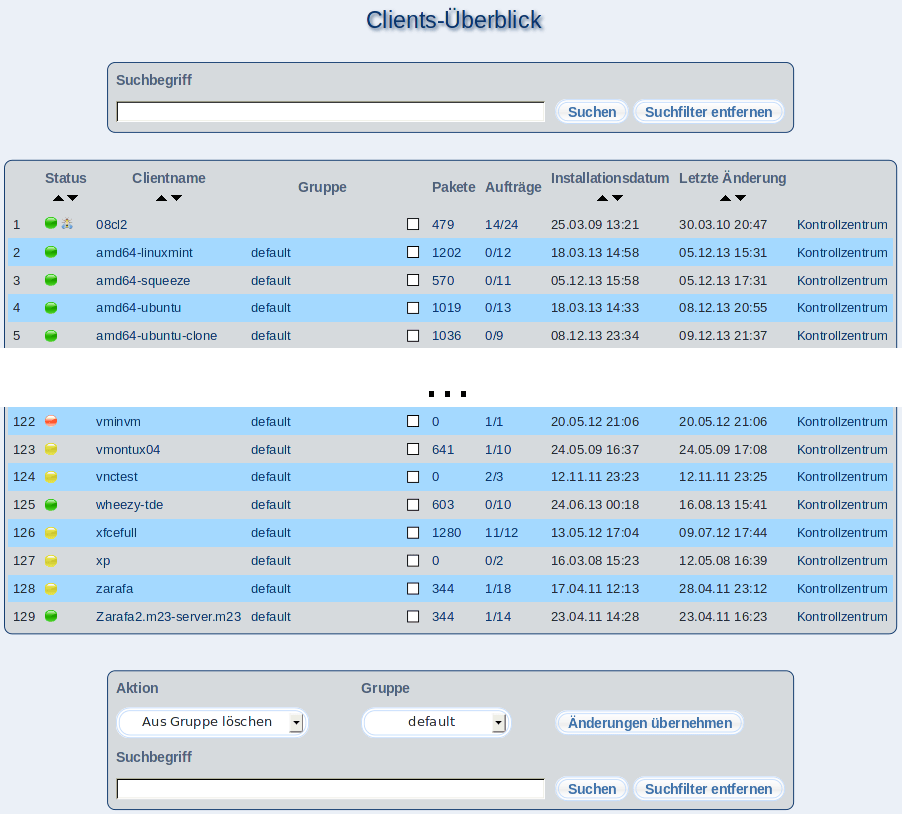
\includegraphics[scale=0.4]{/mdk/doc/manual/screenshots/en/clients_overview.png} \\
If you click on the client name, you get detailed information about the selected client and can enter the control center.\\
\subsection{Status description}
The color marks the installation status of the client.\\
\begin{itemize}
\item \textbf{red}: Client is added, but hardware detection is not complete.\\
\item \textbf{yellow}: Now you can partition and format the client. A base system with graphical user interface is installed automatically.\\
\item \textbf{green}: The base system is installed, now you can add some additional software packages.\\
\item \textbf{blue}: Currently the client installs additional software.\\
\item \textbf{orange}: The client is in the \textbf{critical state}. That means there was an error during installation which must be solved by the administrator. The control center gives you some solution proposals to solve the critical state.\\
\item \textbf{white}: This is a master client for mass installation from whom the settings are transferred to the other clients.\\
\item \textbf{bug}: The bug indicates that the client is in debug mode.\\
\end{itemize}
\subsection{Jobs}
In this row you can see the amount of waiting jobs before and the amount of all jobs after the slash.\\
\subsection{Work on multiple clients}
Select the clients by checking the boxes in the client lines.\\
Now you can work on all selected clients::\\
\begin{itemize}
	\item \textbf{remove from group}: Select the group, all clients should be deleted from. Nothing is done, if a client is not in the selected group.\\
	\item \textbf{add to group}: Select the group, all clients should be added to. Nothing is done, if a client already is in the selected group.\\
	\item \textbf{Delete}: Deletes the selected clients.\\
\end{itemize}
\subsection{Hint}
Use the refresh function of your browser to see the current status of your clients. (e.g. by pressing the F5 key).\\
\subsection{Gimmicks}
\begin{itemize}
\item You can change the status of a client if you click on the according status symbol. You should only change the status if you know what you are doing.\\
\item The debug mode can be (de)activated by clicking the bug icon.\\
\end{itemize}


	%control center
	\input{../clientdetails.hlp.tex}
		\section{Hardware information}Here you can see information about the hardware of the selected client.\\
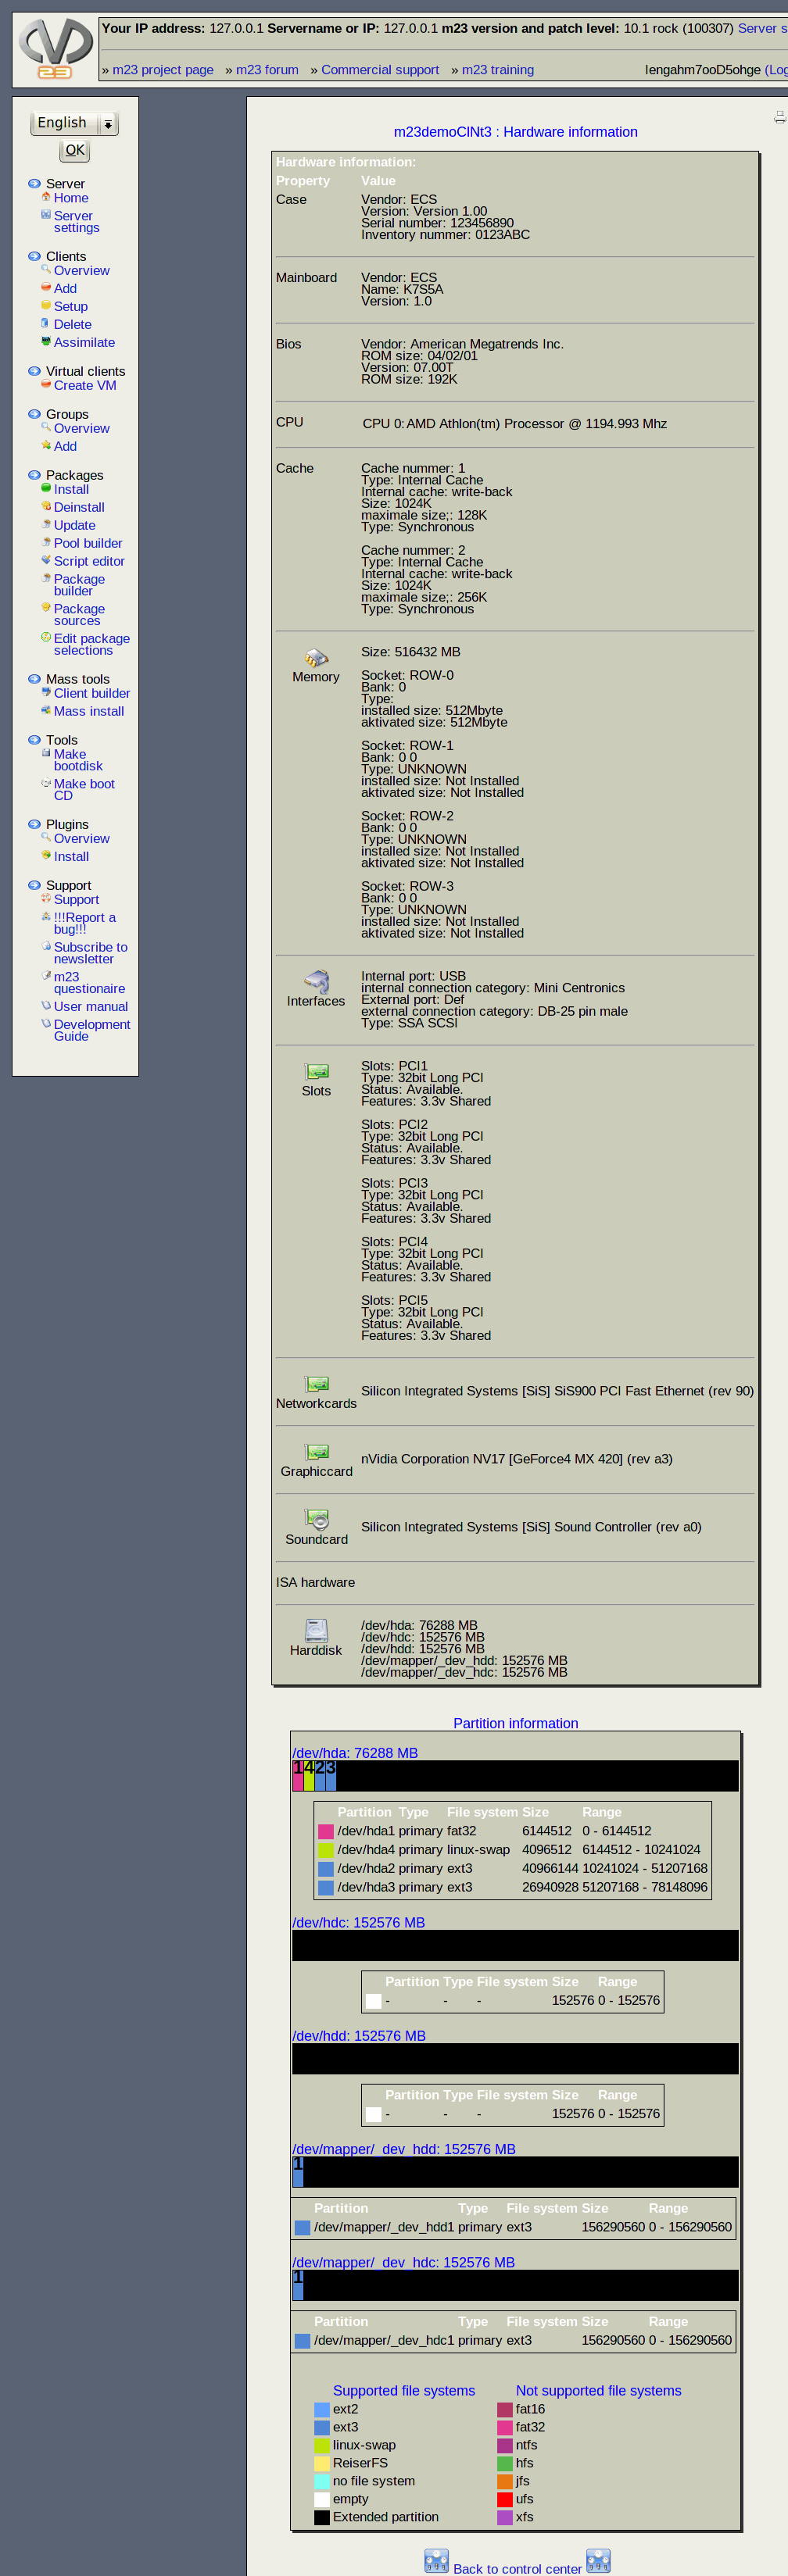
\includegraphics[scale=0.25]{/mdk/doc/manual/screenshots/en/clientinfo_hardware.png} \\

		\section{Paquets}Ici, vous pouvez chercher des paquets qui sont install\'es sur le client. Quand vous voulez voir tous les paquets, n'entrez rien et cliquez sur \textit{$\ll$Rechercher$\gg$}.\\
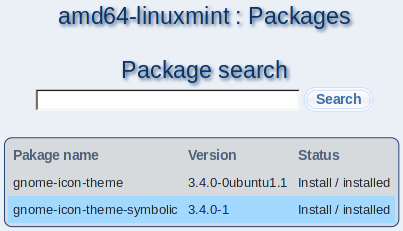
\includegraphics[scale=0.4]{/mdk/doc/manual/screenshots/fr/clients_packages.png} \\

		\section{Client log}This protocol shows you information about installation, deinstallation and other actions.\\
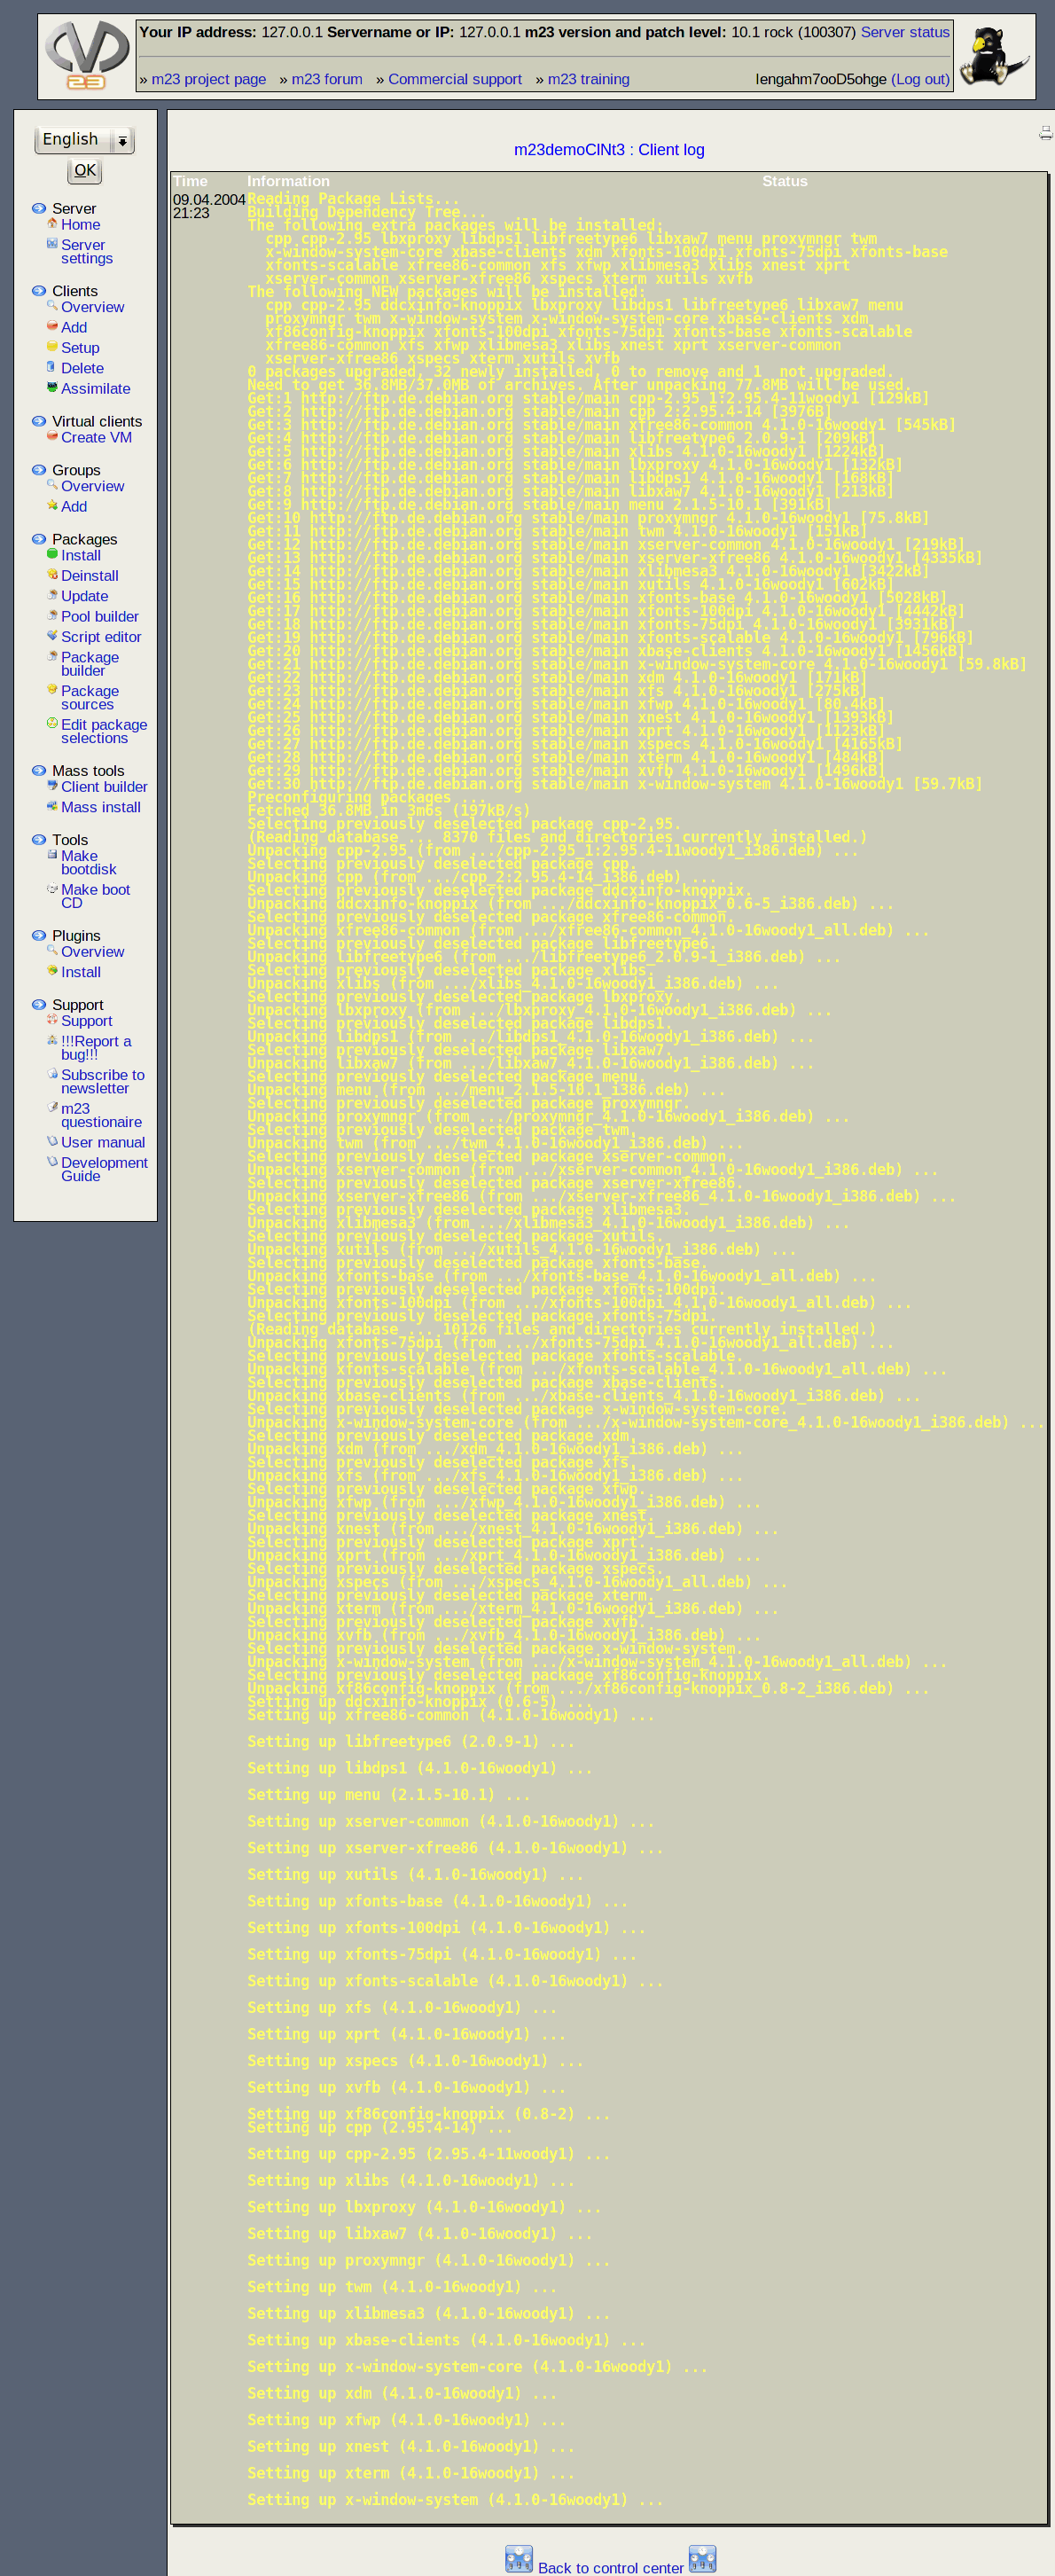
\includegraphics[scale=0.4]{/mdk/doc/manual/screenshots/en/clientinfo_clientLog.png} \\

		\section{Zur Gruppe hinzuf�gen}W�hlen Sie die Gruppen durch Ankreuzen aus, zu denen der Client hinzugef�gt werden soll und klicken anschlie�end auf \textit{"Hinzuf�gen"}.\\
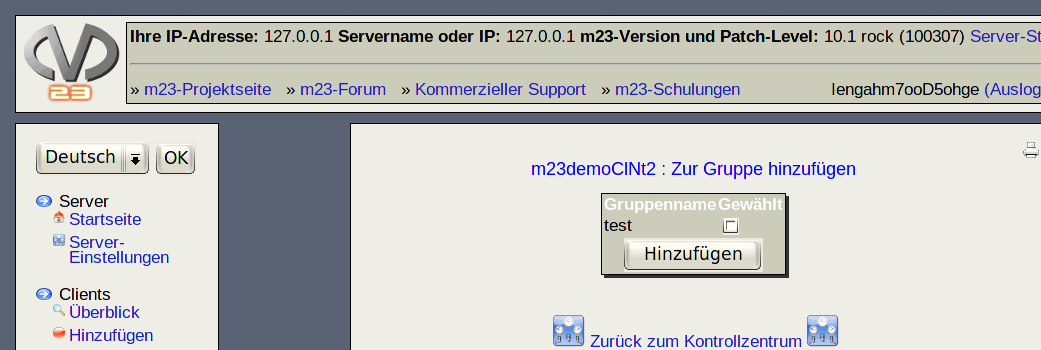
\includegraphics[scale=0.4]{/mdk/doc/manual/screenshots/de/clientinfo_addToGroup.png} \\

		\section{Remove from group}Select the groups by checking you want the client to be deleted from. Click on \textit{"Delete"} afterwards.\\
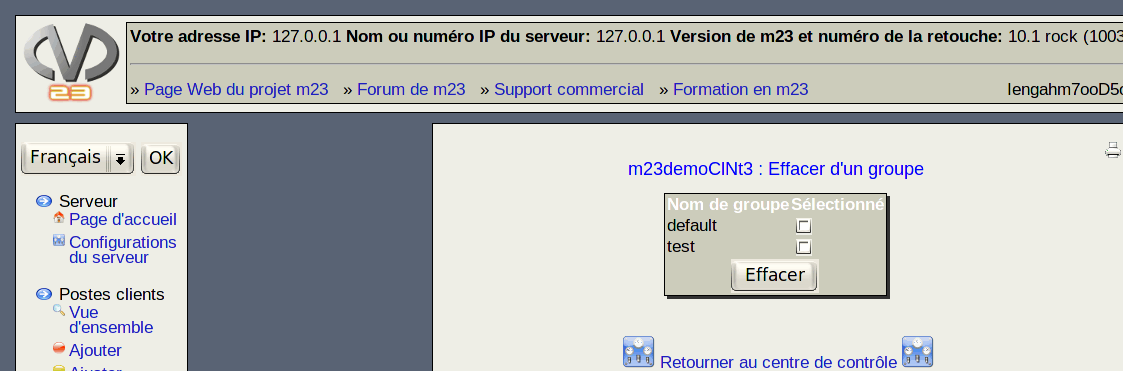
\includegraphics[scale=0.4]{/mdk/doc/manual/screenshots/en/clientinfo_delFromGroup.png} \\

		\section{Client wiederherstellen}Wenn Sie einen Client wiederherstellen, wird er wieder so eingerichtet, wie er installiert wurde. Dies schlie�t Neupartitionierung  und Formatierung mit ein. Es werden alle Softwarepakete neu installiert, die von m23 installiert wurden. Sollten Ver�nderungen am Client per Hand durchgef�hrt worden sein, k�nnen diese nicht wiederhergestellt werden.\\
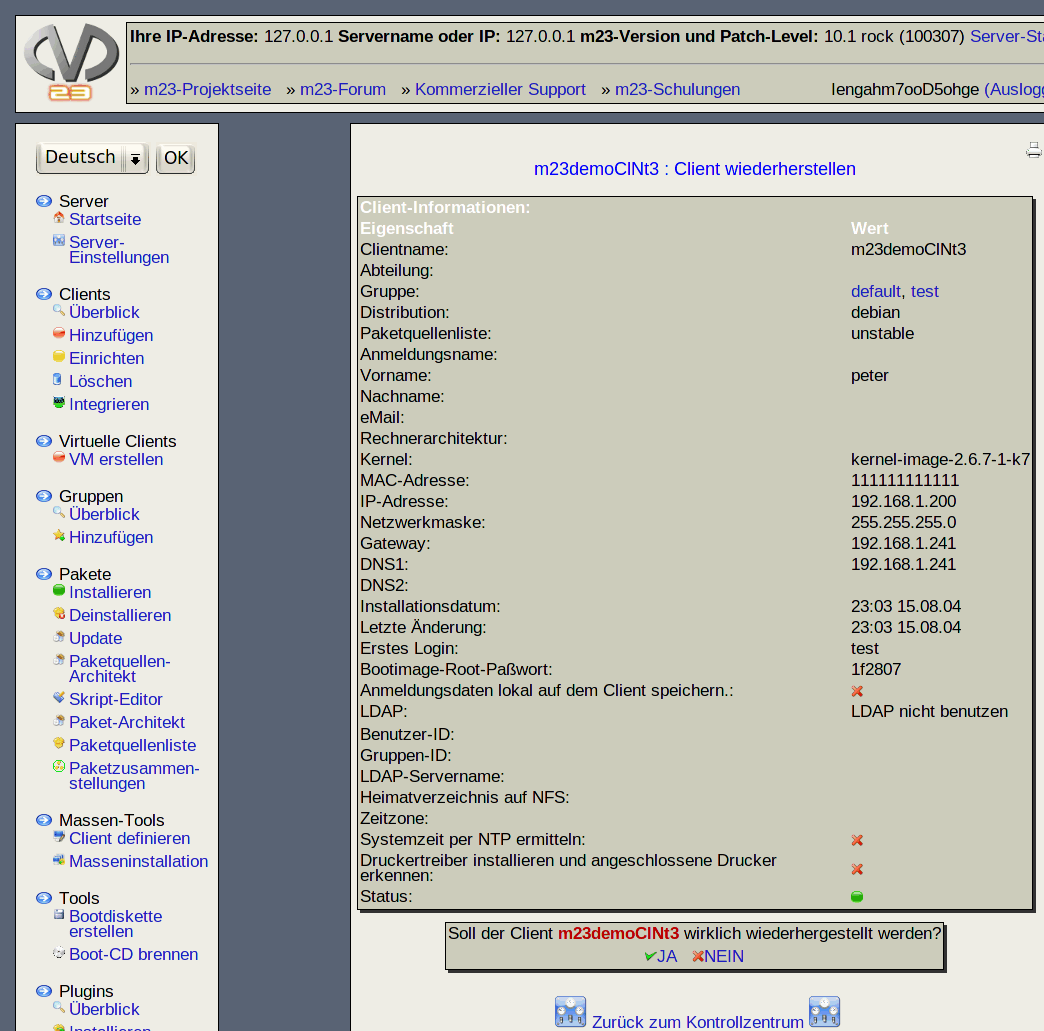
\includegraphics[scale=0.4]{/mdk/doc/manual/screenshots/de/clients_recover.png} \\
\subsection{Hinweis}
Pers�nliche Daten des Client-Benutzers k�nnen nicht wiederhergestellt werden.\\

		\section{Start rescue system}If you want to start a client for repairing or diagnostic purpose, you can boot the rescue system over the network. After the network boot the client starts a console that allows you to do your work. To start the rescue system click on \textit{"Rescue system"} after the client name.\\
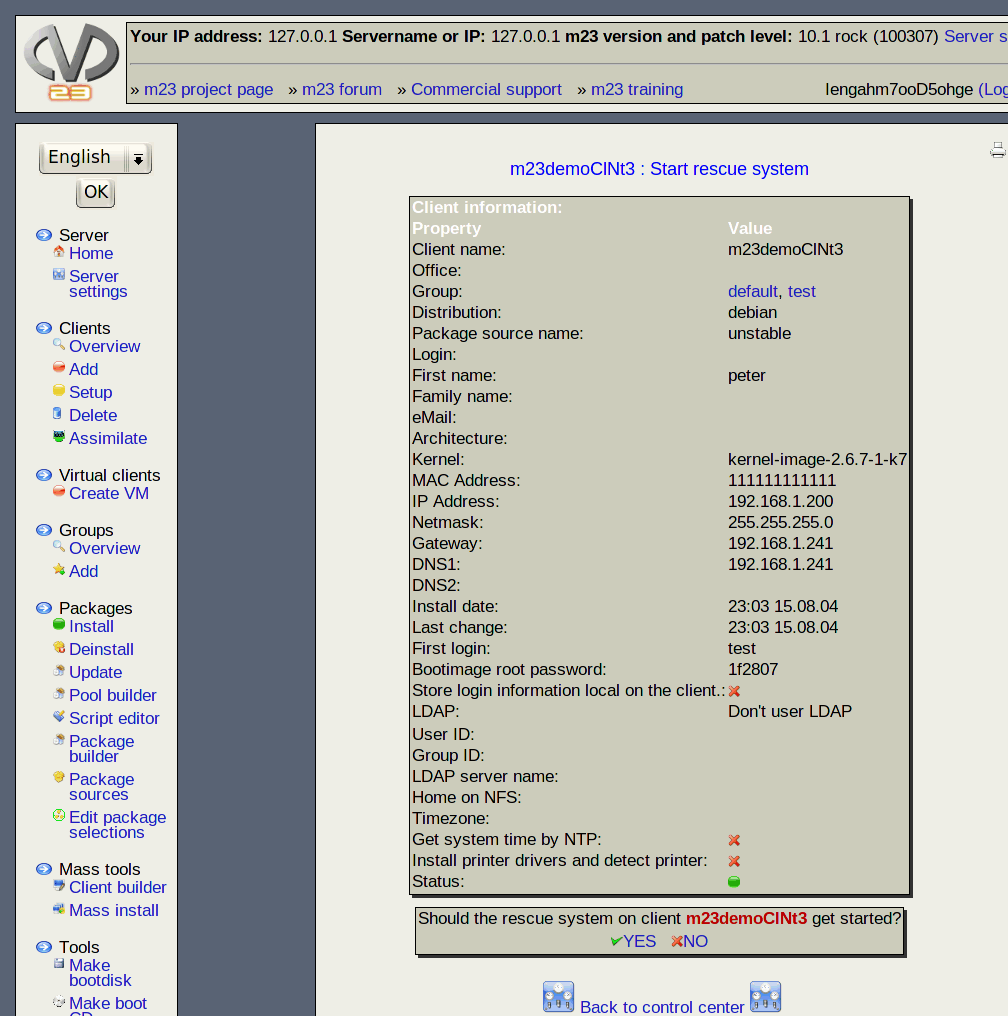
\includegraphics[scale=0.4]{/mdk/doc/manual/screenshots/en/rescue_client.png} \\
\subsection{Hint}:\\
The rescue system will be started every time you boot the client until you delete the "m23Rescue" job from the job list. You can find the list  on the page \textit{"Clients overview"} if you click on the number in the "Jobs" line.\\

		\section{Change client status}You can change the status of the client. This can be useful for debugging or other purposes.\\
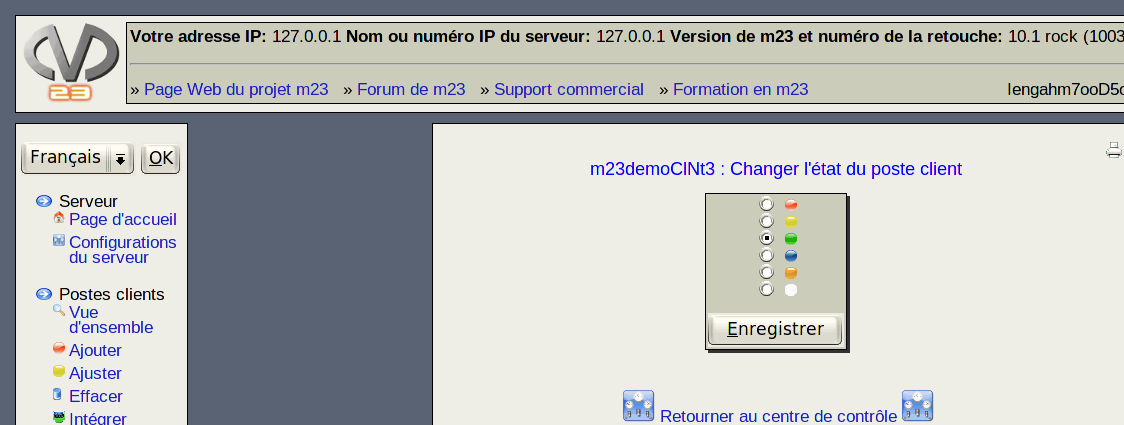
\includegraphics[scale=0.4]{/mdk/doc/manual/screenshots/en/client_status.png} \\
\subsection{Hint}
If you want to change the status, you should know what you are doing.\\

		\section{Changer l'\'etat du d\'ebogage}Des postest client avec le mode de d\'ebogage activ\'e n'indiquent pas d'informations sur l'\'etat de l'utilisateur sur le moniteur, mais les donn\'ees de sortie du script ex\'ecut\'e et des programmes utilis\'es.\\
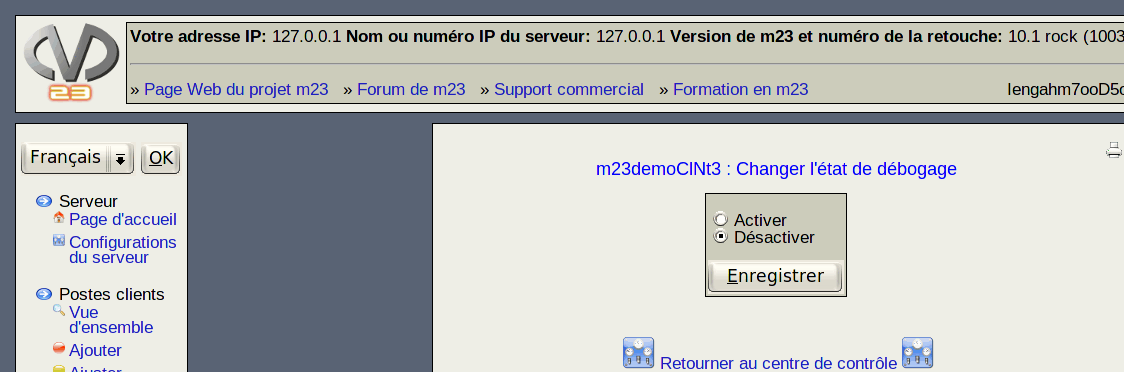
\includegraphics[scale=0.4]{/mdk/doc/manual/screenshots/fr/client_debug.png} \\
Comme �a, vous pouvez mieux voir s'il y a des erreur ex\'ecutant le script.\\

		\section{Client direct connection}A client direct connection can be used to engage in the client installation process, to read the screen contents or for testing and debugging purpose. The connection is done via SSH. That makes it possible to connect with any SSH client.\\

\includegraphics[scale=0.4]{/mdk/doc/manual/screenshots/en/client_directConnection.png} \\
\subsection{Password}
If the client is in an early installation state, the root password for this client is: "NETROOTPWD"\\
Later, it will be the password you entered for root in the client add dialog.\\
If your browser supports the SSH protocol directly, then you can click on the link to connect to the client: ssh://root@CLIENTIP\\
Otherwise open a console and enter the command: \textbf{ssh -o UserKnownHostsFile=/dev/null -l root CLIENTIP}
To read the current client screen or to engage in the running installation use the command: \textbf{screen -x m23install}

		\section{Change client}In this dialog you can change the settings of a client. There are the edit lines you may allready know from the "Add a new client" dialog and three extra rows. These rows are used to select what should happen with the entered values.\\
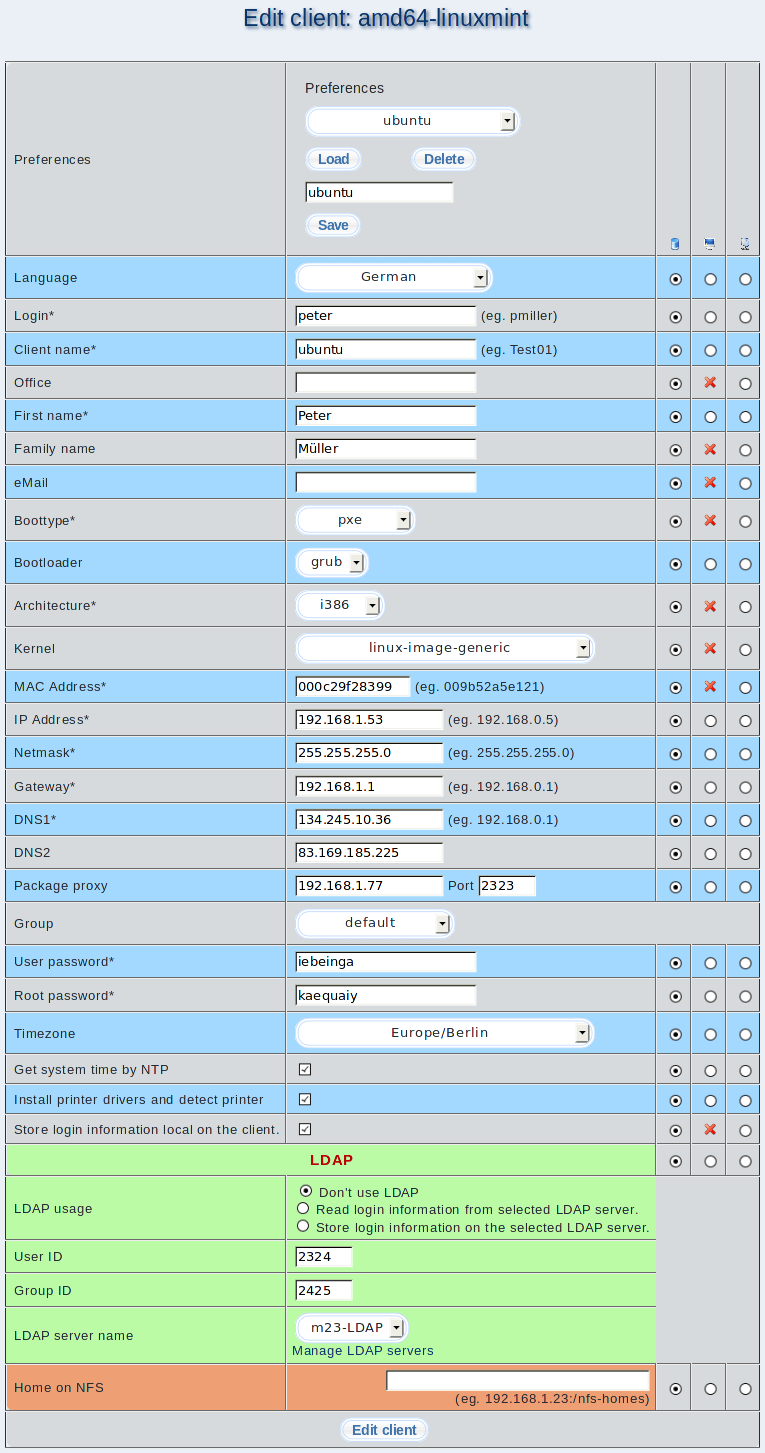
\includegraphics[scale=0.4]{/mdk/doc/manual/screenshots/en/edit_client.png} \\
\begin{itemize}
\item \textbf{Left row}: Select this row if you want to keep the value that is stored on the client and/or the server.\\
\item \textbf{Middle row}: The changes should be made on the client and transferred to the server afterwards.\\
\item \textbf{Right row}: The value is only written to the database on the server. This is useful if you made changes on client side by hand.\\
\end{itemize}
\subsection{Hint}
Some settings are only stored on the server. That's why these settings can't be made on the client. You can't select the middle row on those settings.\\

		\section{Modifier les travaux}Ici, vous pouvez voir les t\^aches du poste client, qui ont d\'ej\`a \'et\'e ex\'ecut\'ees et celles qui attendent leur ex\'ecution et les changer en cas \'echeant. Les possibilit\'es de changement suivantes sont \`a votre disposition:\\
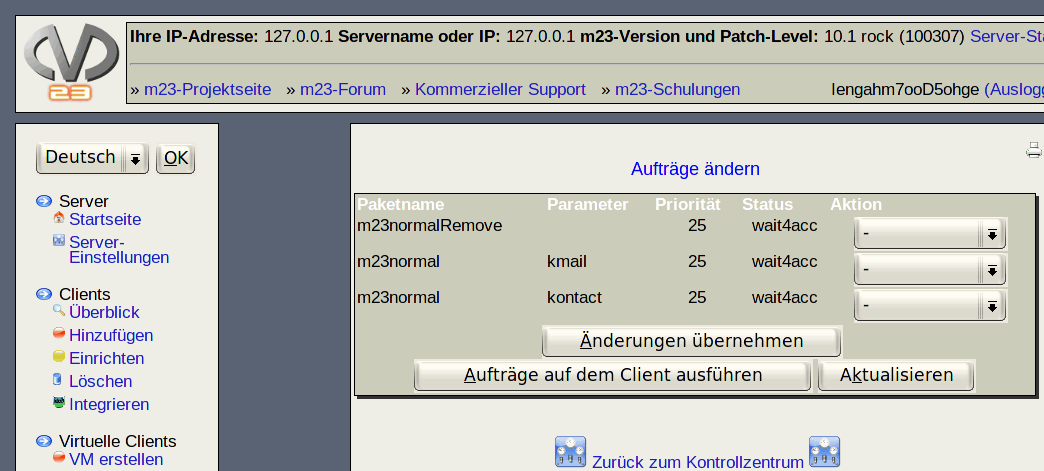
\includegraphics[scale=0.4]{/mdk/doc/manual/screenshots/fr/client_changejobs.png} \\
\begin{itemize}
	\item S\'electionnez \textbf{Effacer} chez \textit{$\ll$Action$\gg$} afin de rejeter la t\^ache d\'efinitivement.\\
	\item \textbf{R�p�ter} d\'eplace une t\^ache d\'ej\`a ex\'ecut\'ee dans la liste des t\^aches \`a accomplir.\\
	\item \textbf{Termin�} marque une t\^ache comme termin\'ee. Celle-ci ne sera plus ex\'ecut\'ee.\\
\end{itemize}
Ensuite, cliquez sur \textit{$\ll$Accepter les changements$\gg$} pour l'enregistrement de vos changements. Si vous voudriez que les t\^aches marqu\'ees avec $\ll$\textbf{R�p�ter}$\gg$ soient ex\'ecut\'ees instantan\'ement, cliquez sur \textit{$\ll$Ex�cuter les travaux sur le poste client$\gg$}.\\

		\section{Cr�er une image}
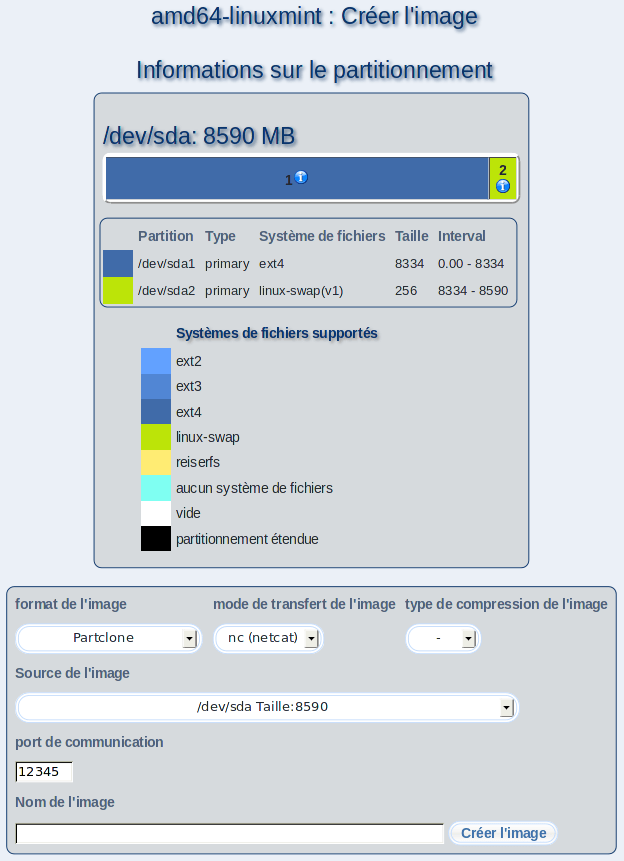
\includegraphics[scale=0.4]{/mdk/doc/manual/screenshots/fr/client_createImage.png} \\
En utilisant ce dialogue, vous pouvez cr\'eer des fichiers image des partitions ou des lecteurs entiers d'un poste client que vous pouvez utiliser pour l'installation des postes client ult\'erieurs. Pour cela, choisissez le format d'image souhait\'e, le mode de transfert de l'image et la compression de l'image. D\'ependant du format de l'image, il est n\'ecessaire que vous entrez des informations additionelles chez \textit{�Source de l'image�}, par exemple quelle partition ou quel lecteur doit \^etre enregistr\'ee dans le fichier image.\\
Puis, choisissez un nom pour votre fichier et entrez-le chez \textit{�Nom de l'image�}. Enfin, cliquez sur \textit{�Cr�er une image�}.\\
\subsection{Les fichiers image}
Les fichiers seront enregistr\'es dans le r\'epertoire \textbf{/m23/data+scripts/clientImages}. Il peuvent \^etre comprim\'es avec des formats diff\'erents et avec des m\'ethodes diff\'erentes. Le sch\'ema de leur nom, quand m\^eme, est toujours le m\^eme: $\langle$nom de l'image$\rangle$$\langle$taille de l'image decomprim\'ee en bytes$\rangle$$\langle$format de l'image$\rangle$$\langle$compression$\rangle$\\
Le format de l'image peut \^etre comme ceci:\\
\begin{itemize}
\item \textbf{dd}: Toutes les donn\'ees d'une partition ou d'un lecteur seront enregistr\'ees.\\
\end{itemize}
Pour la compression, les valeurs suivantes sont valides:\\
\begin{itemize}
\item  (aucune extension de compression): Le fichier image n'est pas comprim\'e.\\
\item \textbf{gz}: La compression sera ex\'ecut\'ee avec le programme gzip.\\
\item \textbf{bz2}: La compression sera ex\'ecut\'ee avec le programme bzip2 (ce qui est plus fort dans la plupart des cas).\\
\end{itemize}
\subsection{La connexion de transfert}
Pour le mode de transfert de l'image, il est n\'ecessaire que vous indiquiez une connexion de r\'eseau qui peut \^etre utilis\'ee de la cot\'e du poste client et du serveur et qui n'est pas bloqu\'ee par un pare-feu etc. Si vous voudriez cr\'eer des plusieures images au m\^eme temps, vous devez choisir des connexions diff\'erentes.\\

		\section{Backup}
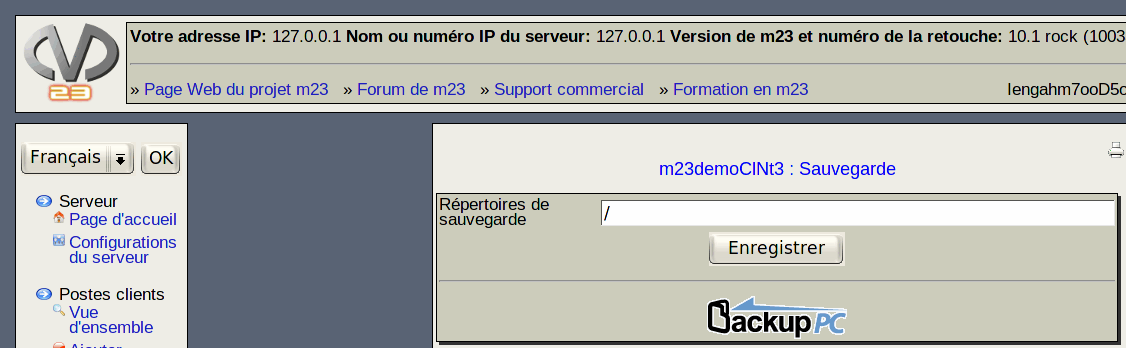
\includegraphics[scale=0.4]{/mdk/doc/manual/screenshots/de/client_backup.png} \\
In diesem Dialog k�nnen Sie alle Verzeichnisse des Clients angeben, von denen ein Backup erstellt werden soll. Geben Sie diese Verzeichnisse dazu durch Kommata getrennt in der Eingabezeile bei \textit{"Backup-Verzeichnisse"} an und klicken Sie anschlie�end auf \textit{"Speichern"}.\\
Das eigentliche Backup �bernimmt das Programm BackupPC, das Sie mit einem Klick auf das Icon starten k�nnen. In der BackupPC-Oberfl�che haben Sie Zugriff auf zus�tzliche Backup-Funktionen.\\

		\input{../poolFromClient.hlp.tex}

\chapter{Clients einrichten} %v1.6
\section{Ajouter un poste client}(les champs de saisie marqu\'ees avec * doivent \^etre remplis correctement en tous cas)\\
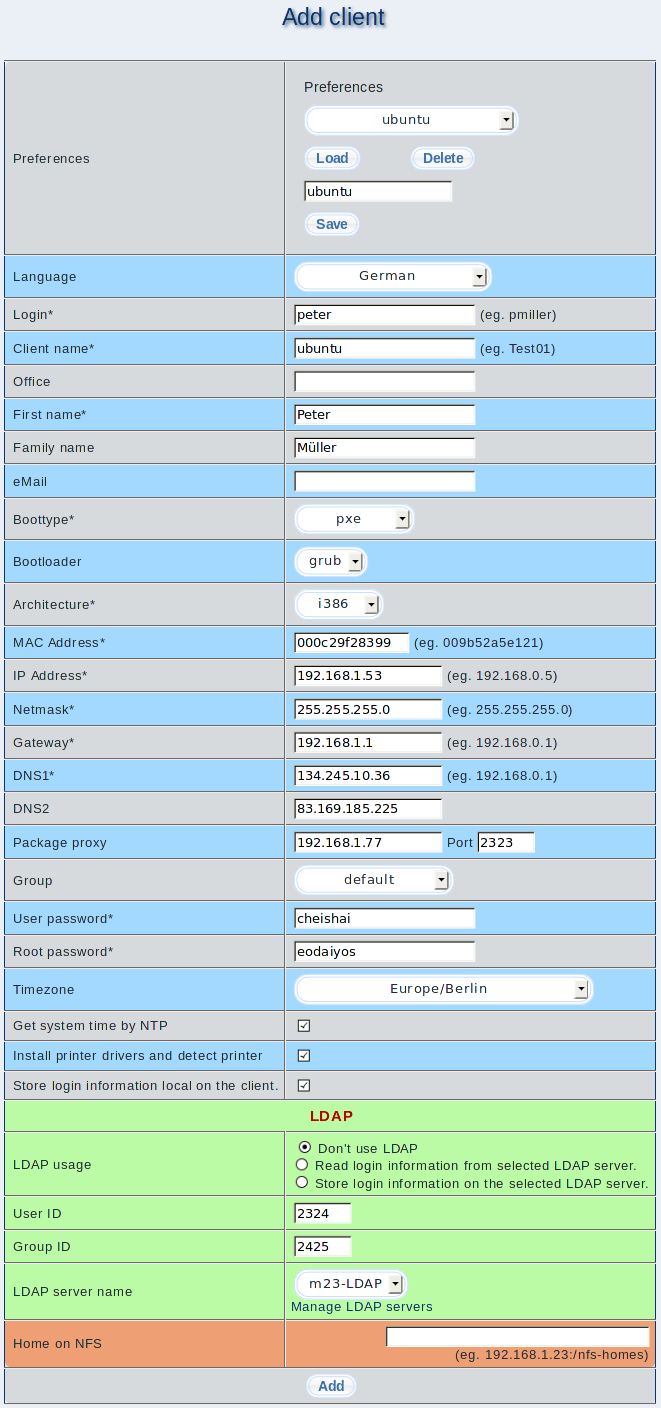
\includegraphics[scale=0.4]{/mdk/doc/manual/screenshots/fr/client_add.png} \\
\begin{itemize}
\item \textbf{Pr�f�rences:} Vous pouvez choisir entre des configurations d\'ej\`a enregistr\'ees et ensuite, vous avez la possibilit\'e de les charger o\`u de les effacer. Si vous voudriez enregistrer la configuration actuelle, entrez un nom pertinent et cliquez sur \textit{$\ll$Enregistrer$\gg$}.\\
\item \textbf{Langue:}Ici vous pouvez choisir la langue pour votre poste client m23. Cette langue sera employ\'ee pour l'ajustement du clavier, du bureau et de la console.\\
\item \textbf{Nom d'entr�e dans le syst�me:} Le nom pour l'entr\'ee dans le syst\`eme du poste client utilis\'e par l'utilisateur.\\
\item \textbf{Nom de poste client:} C'est le nom unique de votre client qui ne devrait pas \^etre employ\'e qu'une fois\\
\item \textbf{Section:} Cette information est volontaire, ici vous pouvez entrer o\`u le client se trouve (par ex. le num\'ero de la chambre etc.)\\
\item \textbf{Langue:} Ici vous pouvez choisir la langue pour votre client. Cette langue sera employ\'ee pour l'installation, pour tous les programmes install\'es, pour le clavier et les options de pays.\\
\item \textbf{Pr�nom:} Pr\'enom de l'utilisateur, correspond au nom d'entr\'ee dans le syst\`eme\\
\item \textbf{Nom de famille:} Nom de famille de l'utilisateur\\
\item \textbf{eMail:} Adresse de courrier \'electronique de l'utilisateur\\
\item \textbf{Type de boot:} Standard de d\'emarrage pour le d\'emarrage des clients vers le r\'eseau. (Notez: Si vous voudriez utiliser m23 avec un serveur DHCP existant, lisez la page suivante: externalDHCP)\\
\item \textbf{Chargeur d'amor�age:} Ici, choisissez quel chargeur d'amor\c{c}age/boot loader vous voudriez utiliser pour l'amor\c{c}age du noyau Linux et des autres syst\`emes d'exploitation eventuellement install\'es. Vous pouvez choisir entre LILO (LInux LOader) et GRUB (GRand Unified Bootloader).\subsection{Information suppl\'ementaire}
La manipulation des param\`etres de d\'emarrage par des personnes non autoris\'ees est emp\^ech\'ee par la protection avec un mot de passe \`a partir de la version m23 0.6.4 . Il est n\'ecessaire d'entrer le mot des passe de d\'emarrage du r\'eseau. Vous pouvez l'extraire dans le centre de contr\^ole sous \textit{$\ll$Connexion directe au poste client$\gg$}.\\
\item \textbf{Architecture du processeur:} Ici, vous pouvez choisir si vous voudriez installer le logiciel pour la version 32 bits ou 64 bits. Regardez aussi le renseignement en bas de la page.\\
\item \textbf{Adresse MAC:} Adresse MAC de la carte r\'eseau du client (par ex. 00:D0:B7:23:86:5C)\\
\item \textbf{Adresse IP:} Adresse IP souhait\'ee du client (par ex. 192.168.1.23)\\
\item \textbf{Masque r�seau:} Masque r\'eseau du r\'eseau (par ex. 255.255.255.0)\\
\item \textbf{Passerelle:} IP de la passerelle pour les connections \`a l'internet ou des autres connections hors du r\'eseau\\
\item \textbf{DNS1:} Adresse IP du serveur DNS pour dissoudre les noms d'internet\\
\item \textbf{DNS2 (facultatif):} Adresse IP du serveur DNS backup\\
\item \textbf{Proxy des paquets:} Le poste client essaie de t\'el\'echarger les paquets de logiciel du num\'ero IP du serveur proxy indiqu\'e. Dans le cas g\'en\'eral, il s'agit du num\'ero IP du serveur m23, mais on peut aussi entrer le num\'ero d'un autre serveur proxy. Si vous laissez ce champs de saisie vide, le client va t\'el\'echarger les paquets de logiciel de l'internet. Entrez \'egalement l'adresse du port du serveur proxy. Au cas du serveur m23, c'est le port 2323. Quand vous ouvrez le dialogue \textit{$\ll$Ajouter un client$\gg$}, le serveur m23 est indiqu\'e comme serveur proxy de standard.\\
\item \textbf{Groupe (facultatif):} Nom du groupe de postes client \`a laquelle appartient le poste client\\
\item \textbf{Mot de passe de l'utilisateur:} C'est le mot de passe de l'utilisateur employ\'e pour la premi\`ere entr\'ee dans le syst\`eme. Ce mot de passe consiste de six chiffres choisis par hasard, mais vous pouvez aussi choisir un autre mot de passe.\\
\item \textbf{Mot de passe de la racine:} C'est le mot de passe qui est employ\'e pour l'acc\`es root au client. Il consiste de huit chiffres choisis par hasard, mais vous pouvez aussi choisir un autre mot de passe.\\
\item \textbf{Fuseau horaire:} Ici, vous pouvez d\'efinir le fuseau horaire, que le poste client doit utiliser.\\
\item \textbf{D�terminer l'heure syst�me par NTP:} S\'electionnez cette option quand vous voudriez que l'heure du poste client doit \^etre accord\'ee par l'internet.\\
\item \textbf{Installer les pilotes de l'imprimante et d�tecter l'imprimante:} Quand vous s\'electionnez cette option, des pilotes d'imprimante seront install\'es et les imprimantes connect\'ees seront d\'etect\'ees.\\
\item \textbf{Enregistrer les donn�es d'ouverture de session local sur le poste client.:}Mettez un crochet ici pour pouvoir utiliser l'entr\'ee dans le syst\`eme locale des postes client.\\
\item \textbf{Ne pas utiliser le LDAP}: Pour pouvoir utiliser l'entr\'ee dans le syst\`eme locale des postes client comme seule option, choisissez \textit{$\ll$Ne pas utiliser le LDAP$\gg$}. \\
\item \textbf{Lire les donn�es d'ouverture de session du serveur LDAP s�lectionn�.}: Si vous voudriez utiliser les donn\'ees d'authentification d'utilisateur enregistr\'ees sur le serveur LDAP, cliquez sur \textit{$\ll$Lire les donn�es d'ouverture de session du serveur LDAP s�lectionn�.$\gg$}.\\
\item \textbf{Enregistrer les donn�es d'ouverture de session sur le serveur LDAP.}: Mais si vous choisissez d'entrer les donn\'ees d'utilisateur indiqu\'ees en haut dans la banque de donn\'ees LDAP du serveur m23 et de les utiliser pour l'entr\'ee dans le syst\`eme sur les postes client, s\'electionnez \textit{$\ll$Enregistrer les donn�es d'ouverture de session sur le serveur LDAP.$\gg$}. Pour pouvoir s\'electionner cette option, il vous faut d'un serveur LDAP avec acc\`es complet, comme les donn\'ees indiqu\'ees en haut seront enregistr\'ees sur le serveur LDAP.\\
\item \textbf{ID de l'utilisateur, ID du groupe}: En plus, vous devez choisir l'\textit{$\ll$ID de l'utilisateur$\gg$} et l'\textit{$\ll$ID du groupe$\gg$} pour l'utilisateur. Ceci est important surtout quand vous voudriez utiliser NFS pour l'enregistrement des r\'epertoires personnels.\\
\item \textbf{Nom du serveur LDAP}: Enfin, vous devez s\'electionner un serveur LDAP de la liste chez \textit{$\ll$Nom du serveur LDAP$\gg$}. Si le serveur LDAP souhait\'e n'y serait pas affich\'e, vous pouvez l'ajouter apr\`es un clic sur \textit{$\ll$Administrer le serveur LDAP$\gg$}.\\
\item \textbf{R�pertoire personnel sur le serveur NFS:} Cette option assure que les donn\'ees d'utilisateur seront enregistr\'ees sur un serveur NFS central, pour qu'elles puissent \^etre acc\'ed\'ees de tout poste client (en combination avec LDAP). Pour activer le NFS, entrez le nom de l'ordinateur ou son adresse IP et le chemin pour l'enregistrement des r\'epertoires personnels, comme par exemple: \\
\begin{verbatim}
192.168.1.42/nfs/home
\end{verbatim}
.\\
\end{itemize}
Veuillez ajouter le client en cliquant sur \textit{$\ll$Ajouter$\gg$}.\\
\subsection{Information suppl\'ementaire:}
Apr\`es \^etre \'etabli, le client parcourt une sequence de d\'etection du mat\'eriel, pendant laquelle des informations, comme par ex. sur la taille du disque dur utilis\'e, sont envoy\'ees au serveur.\\
Apr\`es l'ach\`evement du transfert des donn\'ees l'\'etat du client change \`a \textit{$\ll$jaune$\gg$} et vous pouvez ajuster le client. Pour cela, cliquez sur \textit{$\ll$Postes clients$\gg$} et puis sur \textit{$\ll$Configuration$\gg$} dans le menu.\\
\subsection{Renseignement concernant l'architecture du processeur}
m23 est compatible avec les processeurs 32 et 64 bits. Une version 32 bits peut \^etre install\'ee sur un ordinateur avec 64 bits, \`a l'envers, ce n'est pas possible. Pour profiter du potential entier d'un microprocesseur 64 bits, vous devriez choisir \textit{$\ll$amd64$\gg$}. Parmi la cat\'egorie \textit{$\ll$amd64$\gg$} ne comptent pas seulement les CPUs de AMD, mais aussi ceux de Intel.fallen nicht nur die CPUs von AMD sondern auch die von Intel. Par exemple, les CPUs des Intel Pentium D, Pentium Extreme Edition, Celeron D et Core 2 et les CPUs AMD Sempron, Athlon 64, Athlon X2 et Phenom y appartiennent.\\

	\input{../externalDHCP.hlp.tex}
\input{../clientPartitionFormat.hlp.tex}
\section{Select the client distribution}\subsection{Information:}
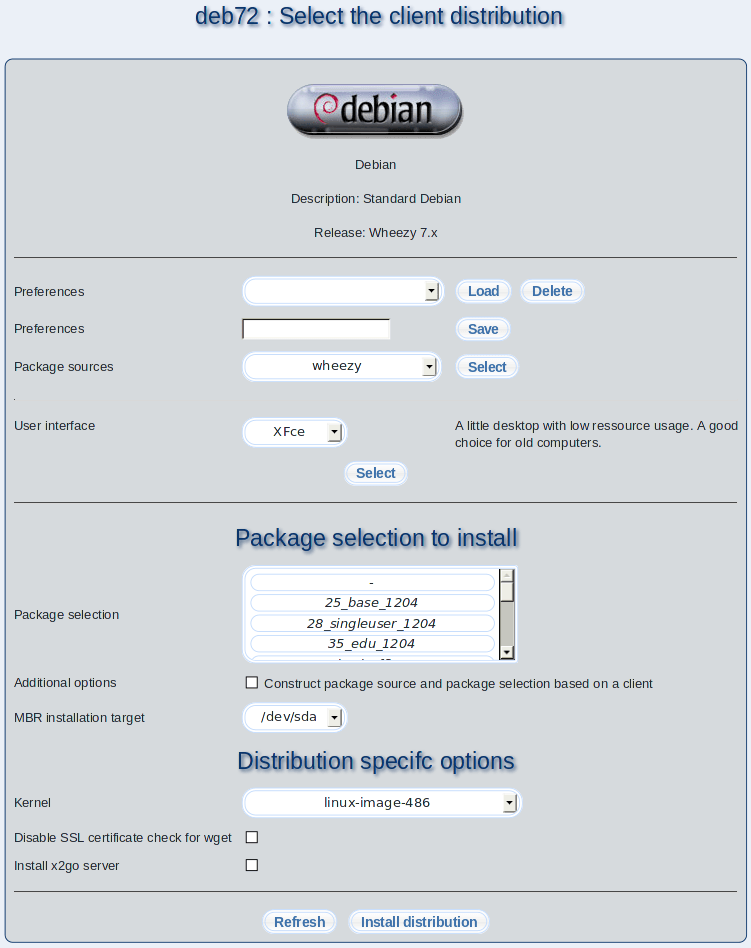
\includegraphics[scale=0.4]{/mdk/doc/manual/screenshots/en/client_distr.png} \\
A distribution is a composition of different software packages stored on CDs, DVDs or in the internet. Some of these distributions are free software and available for free download. E.g. Debian is a free Linux distribution. Distributions differentiate in the installation program and the eye candy of the desktop only. There are no significant differences. The selection of a certain distribution is mostly a matter of taste. This dialog makes it possible to install different distributions with m23.\\
\begin{itemize}
	\item \textbf{Loading preferences}: Select a previously saved preference from the list and click on \textit{"Load"}.\\
	\item \textbf{Deleting preferences}: By clicking on the \textit{"Delete"} button you can remove the selected preference.\\
	\item \textbf{Saving preferences}: You can save the current values as a preference by entering a name and clicking on the \textit{"Save"} button.\\
	\item \textbf{Package sources}: You have to choose the package source first that can be found, created or modified under  \textit{Packages} $\rightarrow$ \textit{Package sources}. Choosing a package selection predefines the Linux distribution and the distribution's release and the installable user interfaces. Click on \textit{"Select"} to choose the package source. The logo and a short descriptive text for the choosen distribution will be shown.\\
	\item \textbf{User interface}: Depending on the selected distribution, you have the choice between different graphical user interfaces (GUIs). If you want to install a server without a graphical desktop you can select \textit{"Textmode"} .\\
	\item \textbf{Package selection}: You can choose a package selection that will be installed together with the operating system.\\
	\item \textbf{MBR installation target}: m23 tries to detect the first harddisk drive for installing the bootmanager automatically. If you want to choose a different disk, you can do it here. Please keep in mind that you have to choose the drive that is the first in the BIOS booting order.\\
	\item \textbf{Distribution specifc options}: Every distribution can define a variety of options which are used during the distribution installation.\\
\end{itemize}
To start the installation simply click on \textit{"Install distribution"}.\\
\subsection{Hint for imaging}
Select \textit{"imaging"} as package sources to install images.\\
You can choose if you want to install a previously created MBR file or the generic bootloader of m23 to the the client's MBR (Master Boot Record). Select the file name or \textit{"Generic MBR"} from the \textit{"Install the generic MBR or the MBR from an image"} list.\\
\subsection{Hint:}
If you save a preference under the same name as a preference for client settings, the distribution settings will be added to the preference. On the other hand, distribution specific preferences will be overwritten.\\

\section{Delete a client}
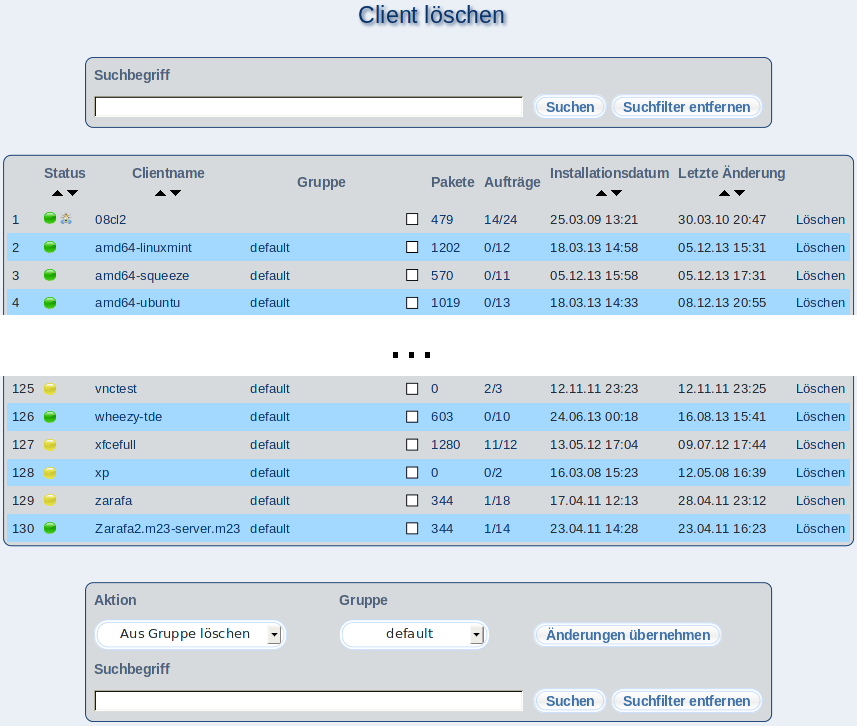
\includegraphics[scale=0.4]{/mdk/doc/manual/screenshots/en/clients_delete.png} \\
To delete a client, click on \textit{"Delete"}. In the following dialog you can see if it is the correct client to delete.\\
If you click on the client name, you get detailed information about the selected client and can enter the control center.\\
\subsection{Status description}
The color marks the installation status of the client.\\
\begin{itemize}
\item \textbf{red}: Client is added, but hardware detection is not complete.\\
\item \textbf{yellow}: Now you can partition and format the client. A base system with graphical user interface is installed automatically.\\
\item \textbf{green}: The base system is installed, now you can add some additional software packages.\\
\item \textbf{blue}: Currently the client installs additional software.\\
\item \textbf{orange}: The client is in the \textbf{critical state}. That means there was an error during installation which must be solved by the administrator. The control center gives you some solution proposals to solve the critical state.\\
\item \textbf{white}: This is a master client for mass installation from whom the settings are transferred to the other clients.\\
\item \textbf{bug}: The bug indicates that the client is in debug mode.\\
\end{itemize}
\subsection{Jobs}
In this row you can see the amount of waiting jobs before and the amount of all jobs after the slash.\\
\subsection{Work on multiple clients}
Select the clients by checking the boxes in the client lines.\\
Now you can work on all selected clients::\\
\begin{itemize}
	\item \textbf{remove from group}: Select the group, all clients should be deleted from. Nothing is done, if a client is not in the selected group.\\
	\item \textbf{add to group}: Select the group, all clients should be added to. Nothing is done, if a client already is in the selected group.\\
	\item \textbf{Delete}: Deletes the selected clients.\\
\end{itemize}
\subsection{Hint}
Use the refresh function of your browser to see the current status of your clients. (e.g. by pressing the F5 key).\\
\subsection{Gimmicks}
\begin{itemize}
\item You can change the status of a client if you click on the according status symbol. You should only change the status if you know what you are doing.\\
\item The debug mode can be (de)activated by clicking the bug icon.\\
\end{itemize}

\section{Client assimilation}
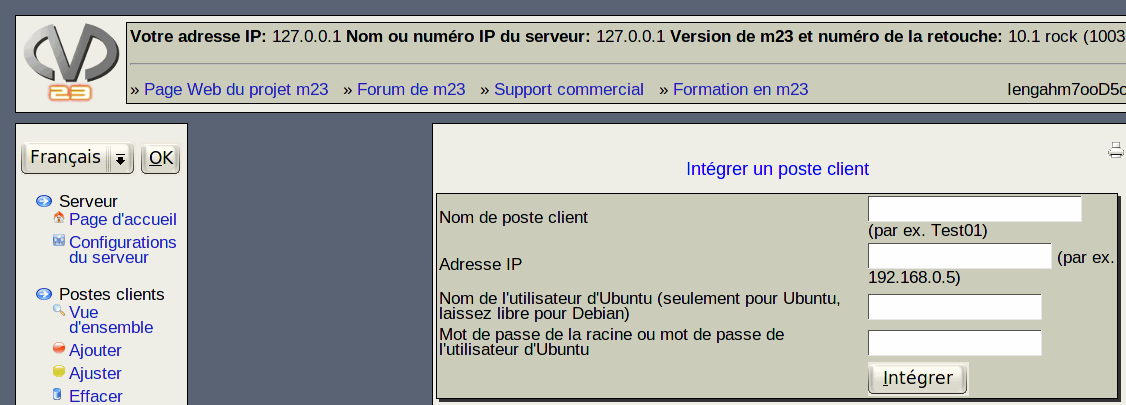
\includegraphics[scale=0.4]{/mdk/doc/manual/screenshots/en/client_assimilate.png} \\
After the assimilation over this dialog you can administrate existing Debian systems with m23. The client must be started up completely and reachable over the network for smooth assimilation. Now you have to enter only three values:\\
\begin{itemize}
\item \textbf{Client name}: This is the name the client should be known by the m23 server. It is advised, but not required to enter the hostname of the client.\\
\item \textbf{IP Address}: This is the (temporary) IP address of the client\\
\item \textbf{Name of the Ubuntu user (only for assimilating Ubuntu systems. Keep empty for Debian)}: Enter here a username that is known to the system and that is allowed to log in via SSH and execute commands via sudo as root with the same password. This is only needed on computers installed with Ubuntu or with disabled root logins.\\
\item \textbf{Root password or password of the Ubuntu user}: This is the current root password of the client or the user password on Ubuntu systems. You can leave empty this field too if you prefer manual intergration.\\
\end{itemize}
Click on \textit{"Assimilate"} afterwards. The assimilation is done in the background.\\
\subsection{Hint}
For automatic assimilation a running SSH daemon that allows logging in as "root" is required on client side. The programm "wget" and the package "coreutils" have to be installed too. And at last it is required that packages can be installed via APT and downloaded from the internet.\\
\subsection{Manual assimilation}
You can start the assimilation by hand if there is no SSH daemon running on the client. Execute the following commands as root in a console on the client (replace "serverIP" with the IP of your m23 server):\\
\begin{verbatim}
cd /tmp; wget http://$\langle$serverIP$\rangle$/work.php -O work.php; sh work.php
\end{verbatim}
\subsection{Hint for the assimilation of an Ubuntu system}
Ubuntu systems can be assimilated normally with "manual assimilation" only, because there is no running SSH daemon . Please start a root console on the Ubuntu system and continue with the hint "Manual assimilation".\\

\input{../makeBootMedia.hlp.tex}


\chapter{Virtualisierung}
\input{../createVM.hlp.tex}
\input{../downloadVBoxAddons.hlp.tex}
\input{../cloudStack.hlp.tex}

\chapter{Gruppenverwaltung}
\section{Gruppen-�berblick}Auf dieser Seite sehen Sie Ihre Client-Gruppen und die Anzahl der jeweils darin enthaltenen Clients. Durch einen Klick auf den Gruppennamen sehen Sie die Detail-Seite der jeweiligen Gruppe.\\
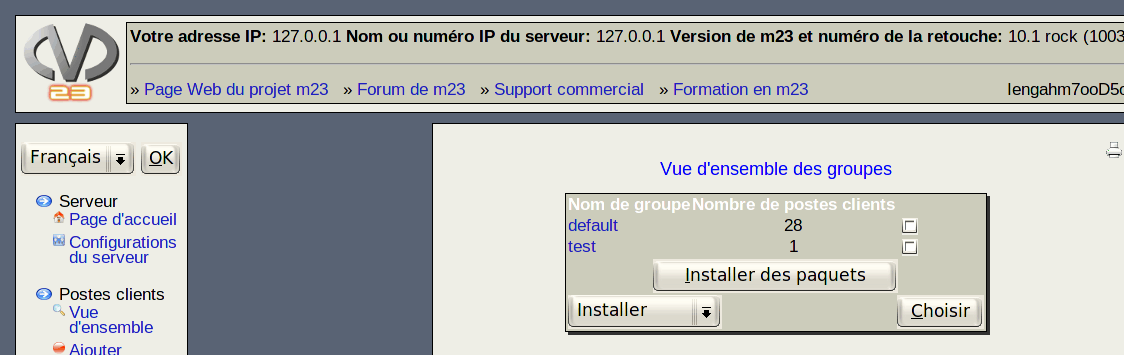
\includegraphics[scale=0.4]{/mdk/doc/manual/screenshots/de/groups_overview.png} \\
\subsection{Auftr�ge an eine Gruppe �bergeben}
Sie k�nnen Auftr�ge an die Clients einer oder mehrerer Gruppen �bergeben und somit die Administration bei der Installation, Deinstallation oder beim Update stark vereinfachen.\\
\subsection{Gehen Sie dazu wie folgt vor:}
\begin{itemize}
\item W�hlen Sie die gew�nschte Aktion aus der Liste.\\
\item Klicken Sie auf \textit{"W�hlen"}, worauf die Beschriftung des Aktions-Buttons die gew�hlte Aktion anzeigen sollte.\\
\item W�hlen Sie die Gruppe(n) aus.\\
\item Klicken Sie schlie�lich 2x auf den Aktions-Button.\\
\end{itemize}

\section{Ajouter un groupe}Ici, vous pouvez ajouter un groupe auquel vous pouvez assigner des postes client. En utilisant des groupes, l'administration de plusieurs postes client avec du logiciel identique est beaucoup facilit\'ee.\\
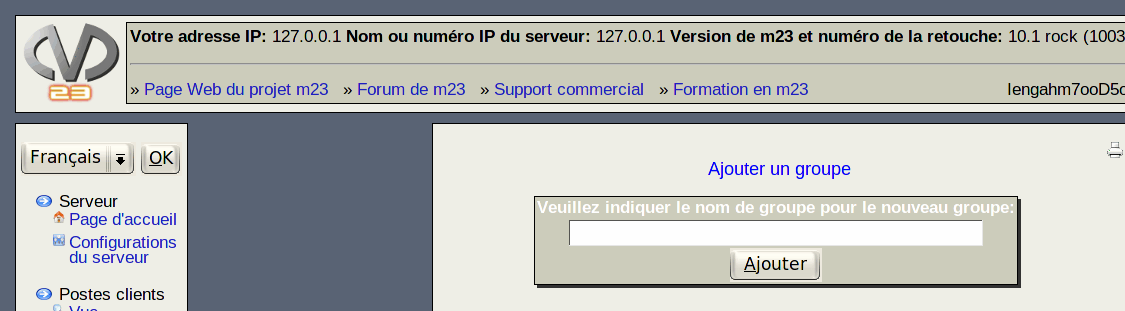
\includegraphics[scale=0.4]{/mdk/doc/manual/screenshots/fr/create_group.png} \\


\chapter{Pakete}
\section{Paketinstallation}
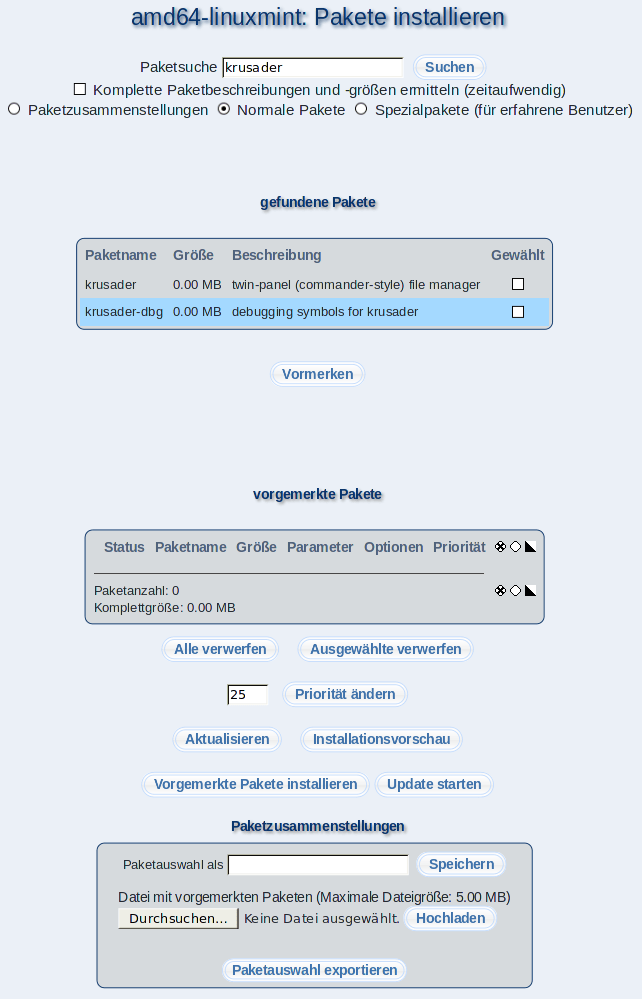
\includegraphics[scale=0.4]{/mdk/doc/manual/screenshots/de/install_packages.png} \\
\subsection{Hinweis}
m23 unterscheidet drei verschiedene Paketarten:\\
\begin{itemize}
\item \textbf{Paketzusammenstellungen:} Sind eine Zusammenstellung von verschiedenen Paketen. Sie k�nnen aus einer Vielzahl von Anwendungen ein Paket schn�ren und so die Installation von identischen Programmpaketen auf verschiedenen Rechnern enorm erleichtern.\\
\item \textbf{Normale Pakete:} Sind normale Programmpakete. Dies sind in der Regel einzelne Programme.\\
\item \textbf{Spezialpakete (f�r erfahrene Benutzer):} Enthalten Pakete, die Spezialaufgaben wie Formatieren etc. durchf�hren. Spezialpakete sollten nur durch erfahrene Benutzer angewendet werden.\\
\end{itemize}
\subsection{Installation von Paketen}
\begin{enumerate}
\item  W�hlen Sie \textit{"Paketzusammenstellungen"}, \textit{"Normale Pakete"} oder \textit{"Spezialpakete (f�r erfahrene Benutzer)"} aus.\\
\item  Geben Sie bei \textit{"Paketsuche"} den Suchbegriff f�r das gew�nschte Paket ein. Lassen Sie das Suchfeld leer, wenn Sie nach allen Pakete einer Paketart suchen m�chten. Dies ist allerdings bei der gro�en Menge der "normalen Pakete" nicht m�glich. Hier mu� ein Suchbegriff angegeben werden.\\
\item  Unter \textit{"gefundene Pakete"} finden Sie alle Pakete, die Ihren Suchparametern entsprechen.\\
\item  Klicken Sie bei den gew�nschten Paketen die Checkbox an.\\
\item  Merken Sie die gew�hlten Pakete durch Klick auf \textit{"Vormerken"} vor.\\
\item  Wiederholen Sie bei Bedarf Schritt 1-5.\\
\end{enumerate}
Nun haben Sie Pakete f�r die Installation vorgemerkt.  Ein gr�ner Haken gibt an, da� dieses Paket zu installieren ist und ein rotes Kreuz, da� dieses Paket vom Client entfernt werden soll. Sie k�nnen die Liste dieser Pakete durch einen Klick auf den Button \textit{"Alle verwerfen"} l�schen oder Pakete ausw�hlen und diese durch \textit{"Ausgew�hlte verwerfen"} entfernen.\\
Schlie�en Sie Ihre Auswahl durch Klick auf \textit{"Vorgemerkte Pakete installieren"} ab.\\
\subsection{Installationsvorschau}
Vor der wirklichen Installation k�nnen Sie �berpr�fen, was die Installation auf dem Client f�r Folgen hat. So k�nnen Sie vorher sehen, welche zus�tzlichen Pakete mitinstalliert werden oder ob es Probleme bei der Installation geben wird. Klicken Sie dazu nach Auswahl der Pakete auf \textit{"Installationsvorschau"}. Nach einiger Zeit sehen Sie ein Protokoll der Installationsvorschau.\\
Eine Installationsvorschau ist allerdings nur dann m�glich, wenn ein einzelner Client und keine Gruppe ausgew�hlt wurde.\\
\subsection{Hinweis zu Paketzusammenstellungen}
Wenn Sie "Paketzusammenstellung" ausw�hlen, k�nnen Sie bestimmen, ob die Pakete auf dem Client installiert oder deinstalliert werden sollen. Au�erdem k�nnen Sie die in der Paketzusammenstellung gespeicherte Aktionen beibehalten. Dies erlaubt es, Installations- und Deinstallations-Auftr�ge in einer einzigen Zusammenstellung zu benutzen. W�hlen Sie dazu aus der Auswahlliste die gew�nschte Aktion aus.\\
\subsection{Tip}
M�chten Sie Ihre Paketauswahl f�r sp�tere Benutzung sichern, geben Sie nach \textit{"Paketauswahl als"} einen Namen f�r Ihre Zusammenstellung ein und sichern Sie diese mit dem \textit{"Speichern"}-Button. Diese Zusammenstellung steht Ihnen sofort unter \textit{"Paketzusammenstellungen"} zur Verf�gung.\\

\section{D\'esinstaller des paquets}Dans ce dialogue, vous avez la possibilit\'e d'effacer des paquets de vos postes client.\\
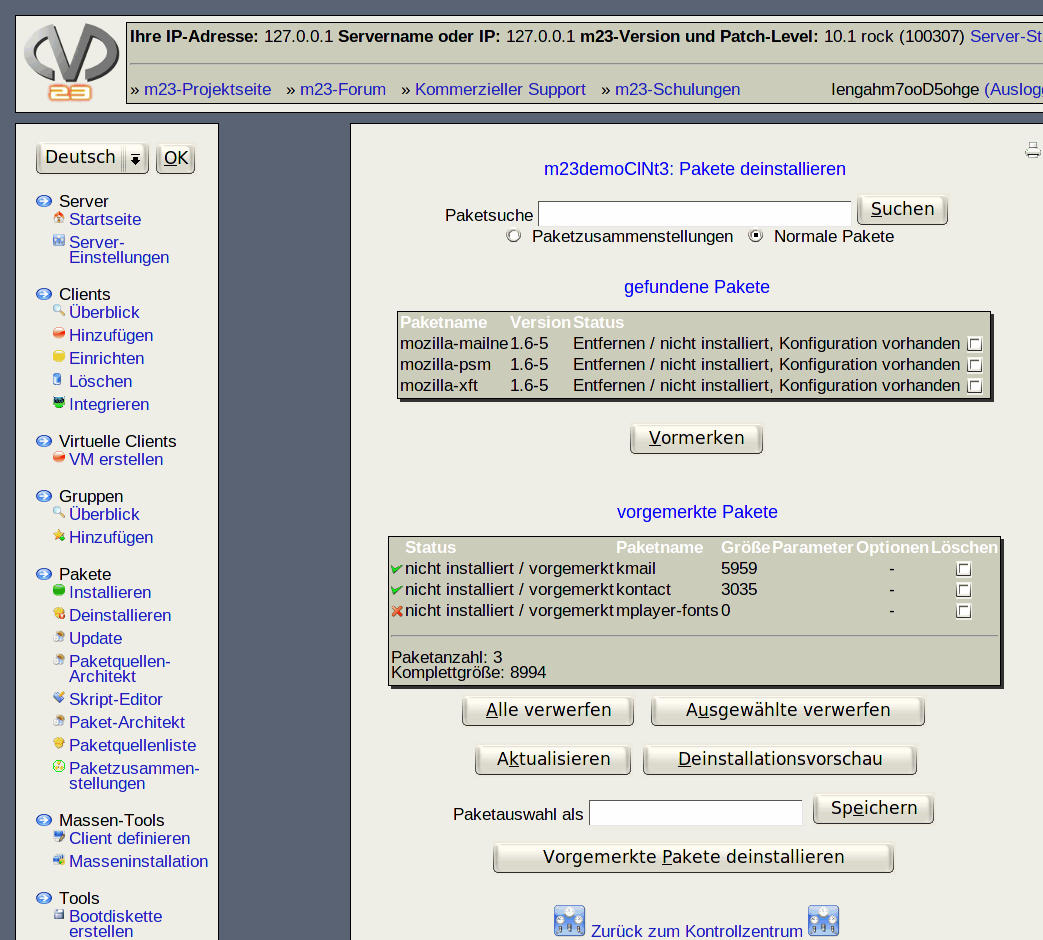
\includegraphics[scale=0.4]{/mdk/doc/manual/screenshots/fr/deinstall_packages.png} \\
\subsection{Notez}
m23 distingue entre trois types de paquet diff�rents:\\
\begin{itemize}
\item \textbf{Combinaisons de paquets:} Ce sont des combinaisons de paquets diff�rents. Vous pouvez empaqueter une quantit� d'applications dans une combinaison de paquets et simplifier l'installation de paquets de programmes identiques sur plusieurs ordinateurs �norm�ment.\\
\item \textbf{Paquets normaux:} Ce sont des paquets de programmes normaux. En g�n�ral, il s'agit des programmes isol�s.\\
\item \textbf{Paquets sp�ciaux (pour utilisateurs exp�riment�s):} Ils contiennent des paquets qui ex�cutent des travaux sp�ciaux comme formater etc., qui devraient �tre utilis�s seulement par des utilisateurs exp�riment�s.\\
\end{itemize}
\subsection{D\'esinstaller des paquets:}
\begin{enumerate}
\item Choisissez $\ll$Combinaisons de paquets$\gg$ ou $\ll$Paquets normaux$\gg$.\\
\item Entrez le mot de recherche pour votre paquet dans le champ de saisie \textit{$\ll$Recherche des paquets$\gg$} ou laissez vide le champ si vous voulez laisser chercher tous les paquets d'un type install\'es sur le poste client.\\
\item Sous \textit{$\ll$Paquets trouv�s$\gg$}, vous voyez tous les paquets qui correspondent \`a vos crit\`eres de recherche.\\
\item Cliquez sur la case \`a cocher derri\`ere les paquets souhait\'es.\\
\item Notez les paquets pour la d\'esinstallation en cliquant sur \textit{$\ll$Noter$\gg$}.\\
\item R\'ep\'etez les \'etapes 1-5 sur vos besoins.\\
\end{enumerate}
Maintenant, vous avez not\'e des paquets pour la d\'esinstallation.  Un crochet vert indique que ce paquet est \`a installer, un croix rouge indique que c'est \`a effacer du client. Vous pouvez effacer la liste de ces paquets en cliquant sur \textit{$\ll$Annuler tous$\gg$} ou s\'electionner des paquets et les effacer apr\`es par un clic sur \textit{$\ll$Annuler la selection$\gg$}.\\
Affirmez votre choix en cliquant sur $\ll$D�sinstaller les paquets not�s$\gg$.\\
\subsection{Pr�vision de la d�sinstallation}
Avant la d\'esinstallation v\'eritable, vous pouvez voir les cons\'equences de la d\'esinstallation pour le poste client. De cette fa\c{c}on, vous pouvez voir auparavant, quels paquets additionels seront d\'esinstall\'es. Pour la pr\'evision, cliquez sur \textit{$\ll$Pr�vision de la d�sinstallation$\gg$} apr\`es que vous avez choisi les paquets. Puis, vous verrez un protocole de la pr\'evision de la d\'esinstallation.\\
Une pr\'evision est seulement possible si vous avez choisi un poste client singulier et pas de groupe.\\
\subsection{Notez: Combinaisons de paquets}
Si vous cliquez sur \textit{$\ll$Combinaisons de paquets$\gg$}, vous pouvez d�cider si les paquets doivent �tre install�s ou d�sinstall�s du poste client. En plus, vous pouvez garder les actions enregistr�es dans la combinaison de paquets. Ceci vous permet d'utiliser des travaux d'installation et de d�sinstallation dans une combinaison singuli�re. Pour cela, choisissez l'action souhait�e de la liste.\\
\subsection{CONSEIL:}
Si vous voulez enregistrer votre choix de paquets pour pouvoir l'utiliser plus tard, entrez un nom pour votre combinaison de paquets apr�s \textit{$\ll$Nom de la combinaison de paquets$\gg$}et cliquez sur \textit{$\ll$Enregistrer$\gg$}. Cette combinaison sera � votre disposition d�s ce moment-l� dans les \textit{$\ll$Combinaisons de paquets$\gg$}.\\

\section{Update}
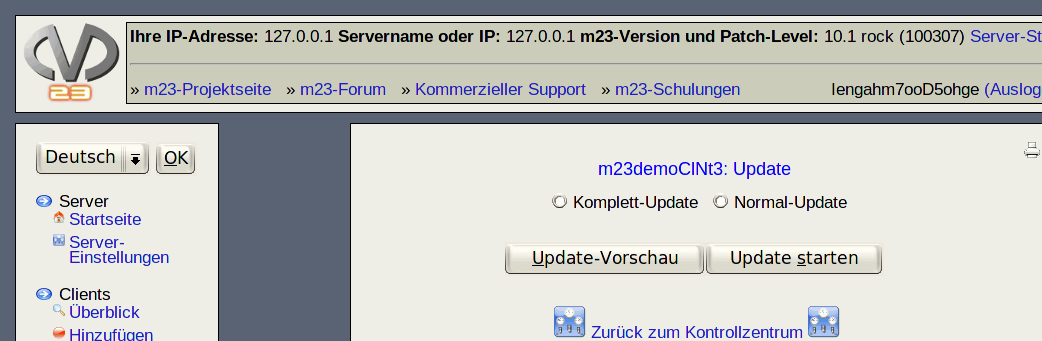
\includegraphics[scale=0.4]{/mdk/doc/manual/screenshots/en/update_packages.png} \\
You can update the software of the client(s) with this update function. If you select a single client you can get a preview of the update procedure.\\
\subsection{Update types}
\begin{itemize}
\item \textbf{Normal update}: Updates installed packages and installs additional packages only, if they are needed.\\
\item \textbf{Full update}: Updates installed packages, new packages are installed and old are removed.\\
\end{itemize}

\input{../autoUpdate.hlp.tex}
\section{Edit package sources}\subsection{Information}
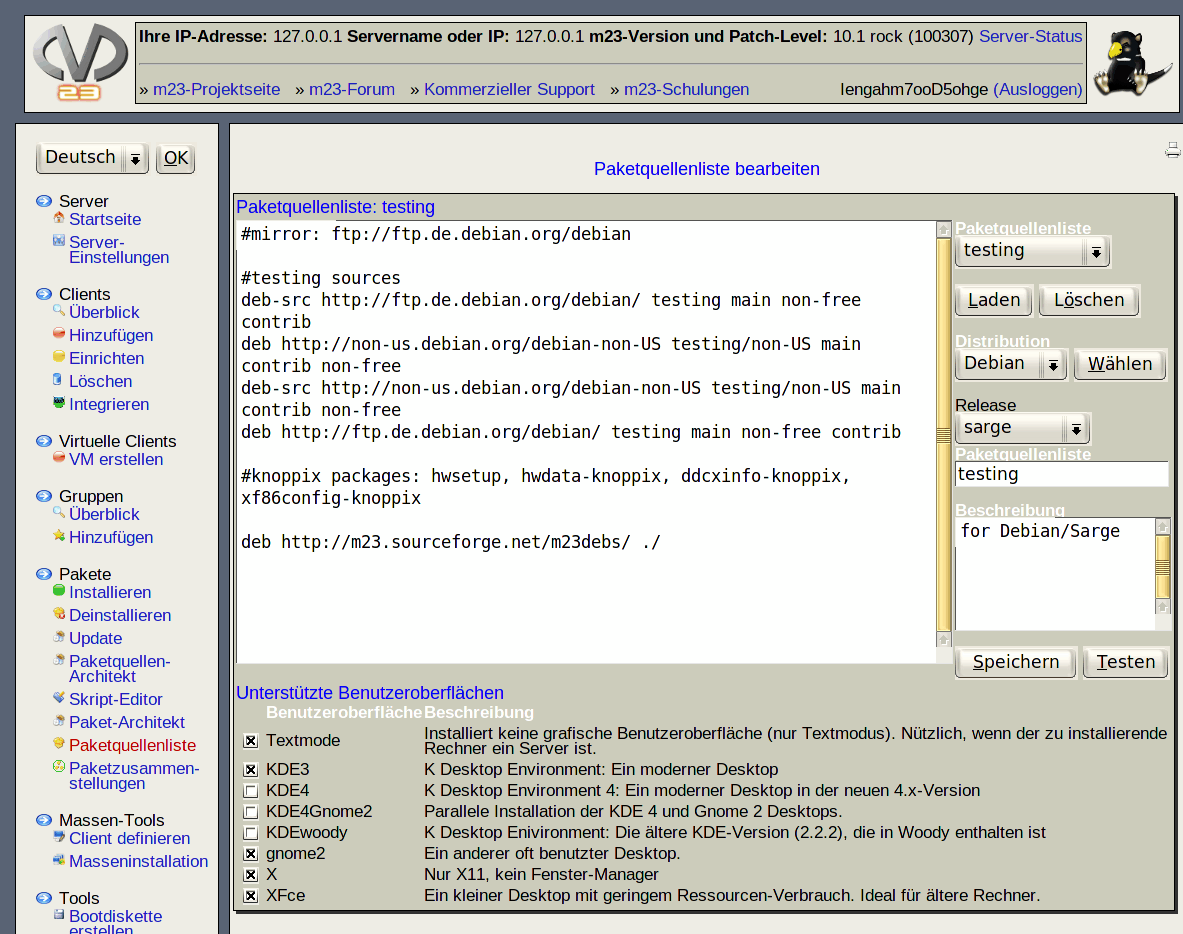
\includegraphics[scale=0.4]{/mdk/doc/manual/screenshots/en/client_sourceslist.png} \\
Software packages can be installed from different sources (HTTP,FTP,CDRom etc.). Different sources are needed, if not all of the software packages can be installed from the same medium. To make it easy for you to administrate these package sources, you can enter them as expected by your selected distribution.\\
\begin{itemize}
	\item \textbf{Loading a package source}: Select a package source from the list (top/right) and click on \textit{"Load"}. The package source will be loaded in the editor.\\
	\item \textbf{Deletion a package source}: To delete the package source loaded in the editor, click on the \textit{"Delete"} button and accept your decision in the next dialog.\\
	\item \textbf{Saving a package source}: The system will always save the package source loaded in the editor. It doesn't matter which package source is selected in the list. Think about a good name for your package source and enter it below \textit{"Pool name"}. If you have loaded a package source before, the package source name is written into the field \textit{"Pool name"} automatically. If you want, you can enter a comment into the \textit{"Description"} text field. Afterwards, click on the \textit{"Save"} button.\\
	\item \textbf{Test the package source}: After entering a package source list, you should test if all sources are working properly. Simply click on the \textit{"Test"} button. The package description files will be downloaded and a test report will be shown thereafter. It can take minutes until the report is shown, depending on your internet connection speed and the speed of the used software package servers.\\
	\item \textbf{Select Mirror}: If you would like to use a different mirror (the standard server is ftp.debian.org) for the installation of the base system, enter it as follows in a new line of your package source: \\
\begin{verbatim}
#mirror: [URL to the packages]
\end{verbatim}
. \textit{URL to the packages} describes the protocol, the hostname or the IP and the directory that contains the packages. A valid URL may look like this: \\
\begin{verbatim}
#mirror: http://192.168.7.14/debianCDs
\end{verbatim}
.\\
\end{itemize}
\subsection{Hint}
\begin{itemize}
\item If you save a package source under a name that already exists, the old package source will be overwritten with the contents of the editor.\\
\item \textbf{Benutzeroberfl�chen} sind direkt an eine Paketquellenliste gebunden. D.h. wenn Sie eine bestimmte Paketquellenliste f�r einen Client benutzen, k�nnen Sie nur die Benutzeroberfl�chen verwenden, die Sie in diesem Dialog f�r die Paketquellenliste freigeschaltet haben. Sie sollten hier deshalb nur die Benutzeroberfl�chen ausw�hlen, die garantiert von den Paketquellen unterst�tzt werden.\\
\end{itemize}

\input{../editPackageSelection.hlp.tex}
\input{../packageBuilder.hlp.tex}
\input{../scriptEditor.hlp.tex}

\chapter{Paketquellenarchitekt}
\input{../poolBuilderCreateEditDelete.hlp.tex}
\input{../poolBuilderReadCD.hlp.tex}
\input{../poolBuilderCreateIndex.hlp.tex}
\input{../poolBuilderSelectPackageSourcesAndPackages.hlp.tex}
\input{../poolBuilderStartDownload.hlp.tex}
\input{../poolBuilderDownloadStatus.hlp.tex}
\input{../poolBuilderShowSourcesList.hlp.tex}

\chapter{Masseninstallation}
\input{../clientBuilder.hlp.tex}
\input{../diskDefine.hlp.tex}
\section{D\'eterminer la m\'ethode de d\'etermination de valeurs}
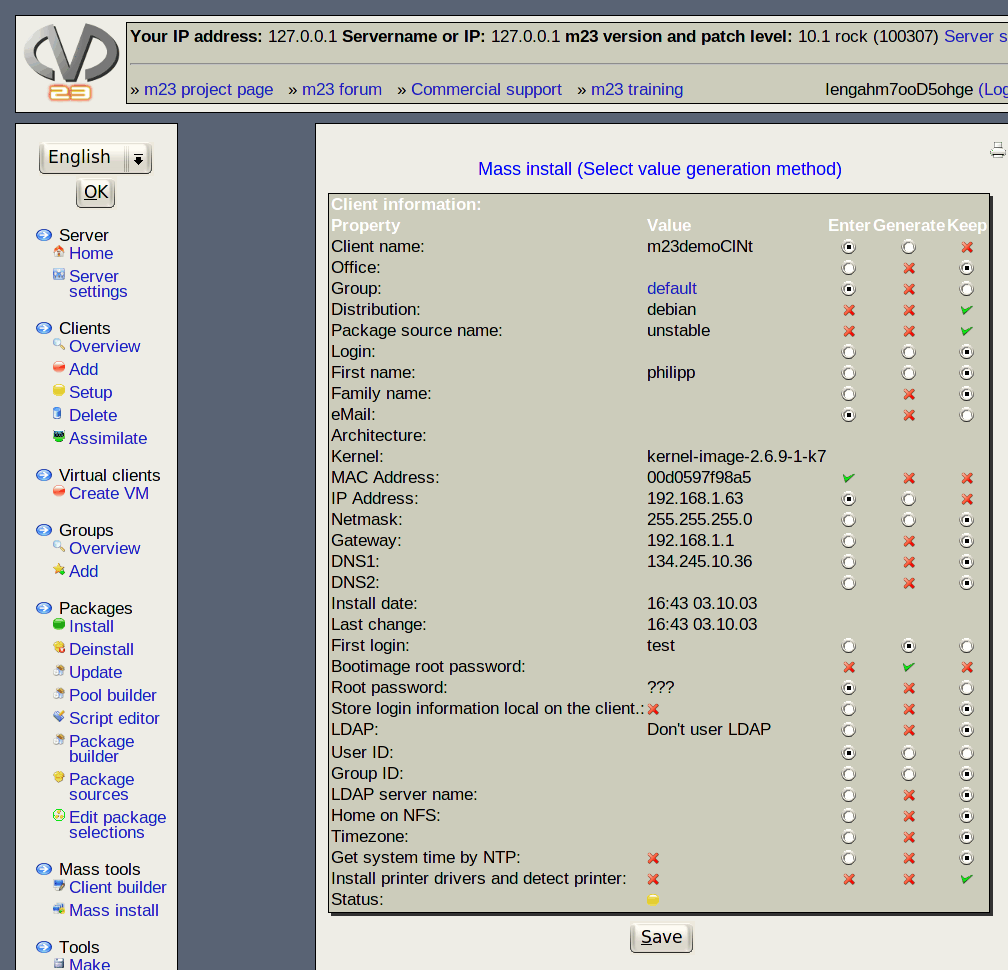
\includegraphics[scale=0.4]{/mdk/doc/manual/screenshots/fr/mi_step0.png} \\
Ici, vous pouvez d\'eterminer comment les valeurs des propri\'et\'es des clients doivent \^etre g\'en\'er\'ees. \\
\subsection{Vous pouvez choisir entre trois m\'ethodes:}
\begin{itemize}
\item \textbf{Entrer}: Vous entrez les propri\'et\'es \`a la main ou par un fichier.\\
\item \textbf{G�n�rer}: Les valeurs seront g\'en\'er\'ees automatiquement. Par exemple, les noms des postes client peuvent \^etre g\'en\'er\'es avec des num\'eros d'ordre ou des adresses IP libre seront utilis\'es.\\
\item \textbf{Garder}: La valeur d\'etermin\'ee pour le $\ll$poste client mod\`ele$\gg$ sera gard\'ee pour tous les postes client.\\
Chez certaines propri\'et\'es, votre choix est limit\'ee. Les m\'ethodes que vous ne pouvez pas choisir sont marqu\'ees avec une croix rouge. Un crochet vert signifie que c'est la seule m\'ethode de d\'etermination de valeurs possible. Par exemple, une adresse MAC ne peut pas \^etre g\'en\'er\'ee, ni \^etre la m\^eme pour tous les postes client. Elle doit \^etre entr\'ee \`a la main ou charg\'ee d'un fichier.\\
\end{itemize}

\section{Datenquelle w�hlen}
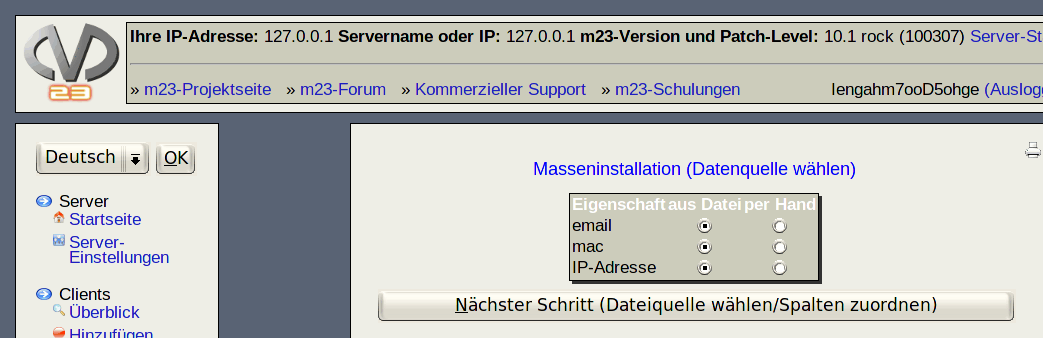
\includegraphics[scale=0.4]{/mdk/doc/manual/screenshots/de/mi_step1.png} \\
W�hlen Sie die Quelle f�r die Eigenschaften aus, die eingegeben werden sollen. Die Werte k�nnen in einer Textdatei vorliegen oder per Hand eingegeben werden.\\

\section{Select data source/Assign columns}
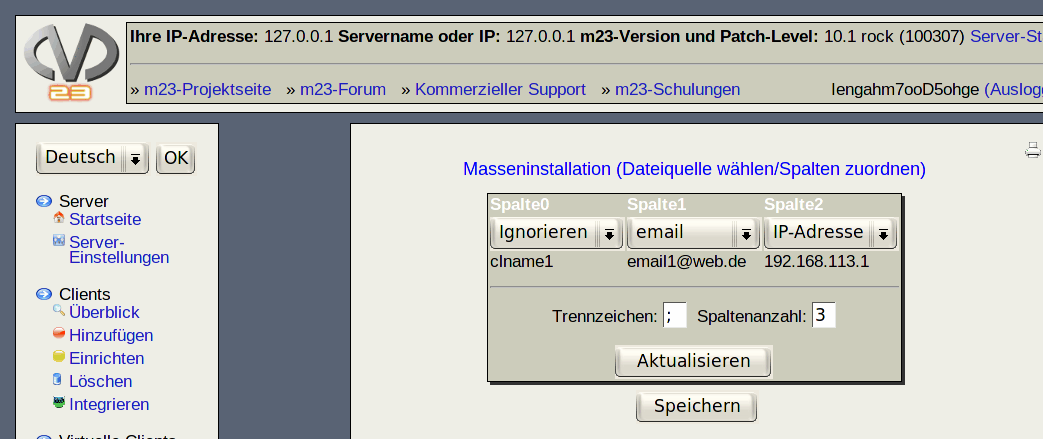
\includegraphics[scale=0.33]{/mdk/doc/manual/screenshots/en/mi_step2.png} \\
This dialog is divided into two steps:\\
\begin{itemize}
\item Select and upload a database file\\
\item Assign the fields to the client options\\
\end{itemize}
\subsection{Select and upload a database file}
Select a file with the diealog and click on \textit{"Upload"}.\\
A special data format is needed to make the value recognition possible for m23. The values for a single client are specified in every line. The client options are separated by a separator character (here ";")::\\
\begin{verbatim}
option1;option2;option3;...
\end{verbatim}
You can use other combinations of a maximum of 4 characters. The order of the options has to be the same in all lines.\\
\subsection{Hint}
All in the file stored values have to be valid and there are an additional requirements for special options:\\
\begin{itemize}
\item \textbf{Store login information local on the client.}: Set it to "yes" if you want to activate this option. All other values disable it.\\
\item \textbf{LDAP}: Here three different values are possible:\\
\begin{itemize}
\item "none": Don't user LDAP\\
\item "read": Read login information from selected LDAP server.\\
\item "write": Store login information on the selected LDAP server.\\
\end{itemize}
\end{itemize}
\subsection{Assign the fields to the client options}
You can assign the fields to the option names after uploading a file.\\
\subsection{Step by step}
\begin{enumerate}
\item Enter the separator character in the separator field and adjust the column amount if needed.\\
\item Click on \textit{"Refresh"}. The first line of the database file is now separated and shown in the client option fields.\\
\item Assign the separated parts from the database file to the client options by selecting the client option names from the selection list.\\
\item End the dialog with a click on \textit{"Save"}.\\
\end{enumerate}

\section{Generator-Optionen}
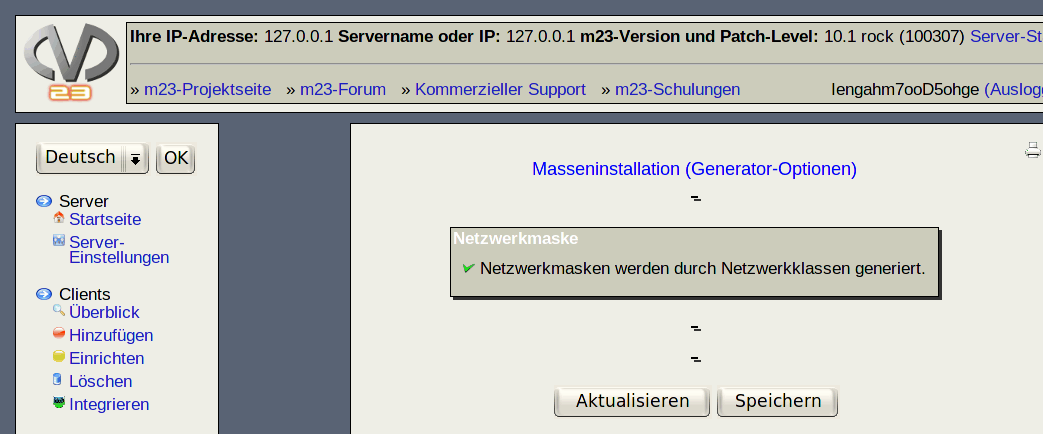
\includegraphics[scale=0.4]{/mdk/doc/manual/screenshots/de/mi_step3.png} \\
Hier k�nnen Sie die Parameter f�r die Generatoren der folgenden Eigenschaften festlegen:\\
\begin{itemize}
\item \textbf{Clientname}: Sie k�nnen hier den Client-Basis-Namen und eine Startnummer vorgeben. Die Clientnamen werden dann in der ben�tigten Anzahl nach dem Schema $\langle$Client-Basis-Name$\rangle$$\langle$fortlaufende Nummer$\rangle$ erstellt. Bereits vergebene Client-Namen werden bei der Generierung �bersprungen. Bsp.: Client-Basis-Name=m23client, Startnummer=12 generiert die Clientnamen m23client12, m23client13, ...\\
\item \textbf{Anmeldungsname}: Dies ist der Name, mit dem sich der Benutzer am Client anmelden kann. Es stehen zwei Methoden zur Generierung zur Verf�gung. Die inkrementelle Variante verh�lt sich identisch zur Erstellung bei \textit{"Clientname"}. Zus�tzlich ist das Bilden aus dem ersten Buchstaben des Vornamens und dem vollst�ndigen Nachnamen m�glich (\textit{"Aus Vor- und Nachnamen erstellen"}).\\
\item \textbf{Vorname}: Die Generierung der Vornamen (die zugleich die Loginnamen sind) geschieht analog zu den Clientnamen.\\
\item \textbf{IP-Adresse}: Legen sie hier die IP-Adressen-Bereiche fest, in denen nach freien IP-Adressen gesucht werden soll. Standardm��ig werden nur IP-Adressen generiert, die nicht bereits von m23-Clients benutzt werden. Sie k�nnen aber auch angeben, da� jede IP-Adresse vor der Verwendung "angepingt" werden soll. Sollte sich unter einer oder mehreren IP-Adressen ein Rechner melden, so werden diese IPs nicht verwendet.\\
\item \textbf{Netzwerkmaske}: Die Netzwerkmasken werden automatisch nach Schema der Netzwerk-Klassen berechnet. Dieses ist per Definition folgenderma�en:\\
\begin{tabular}{|c|c|c|}
\hline
Von & Bis & Netzwerkmaske\\
	 \hline
0.0.0.0 & 127.255.255.255 & 255.0.0.0\\
	 \hline
128.000.000.000 & 191.255.255.255 & 255.255.0.0\\
	 \hline
192.000.000.000 & 255.255.255.255 & 255.255.255.0\\
	 \hline
\end{tabular}
\item \textbf{Erstes Login}: F�r dieses Login k�nnen die Pa�w�rter komplett zuf�llig (\textit{"Zufalls-Pa�w�rter"}) oder nach einem zuf�lligen aber f�r Menschen leichter merkbaren Schema (\textit{"PwGen-Pa�w�rter"}) angelegt werden. Au�erdem kann die L�nge der generierten Pa�w�rter zwischen 6 und 8 Zeichen L�nge variiert werden. Es wird empfohlen, die voreingestellte L�nge von 8 beizubehalten.\\
\item \textbf{Benutzer-ID}: Legen Sie hier die Startnummer fest, ab der freie Benutzer-IDs gesucht und verwendet werden sollen.\\
\item \textbf{Gruppen-ID}: Legen Sie hier die Startnummer fest, ab der freie Gruppen-IDs gesucht und verwendet werden sollen.\\
\end{itemize}

\section{Restliche Werte eingeben/�bersicht}Hier sehen Sie die �bersicht �ber alle zu erstellenden Clients. Nun k�nnen Sie die L�cken in den Tabellen f�llen bzw. Werte �ndern und �berpr�fen, ob die vorhandenen Werte Ihren Vorstellungen entsprechen.\\
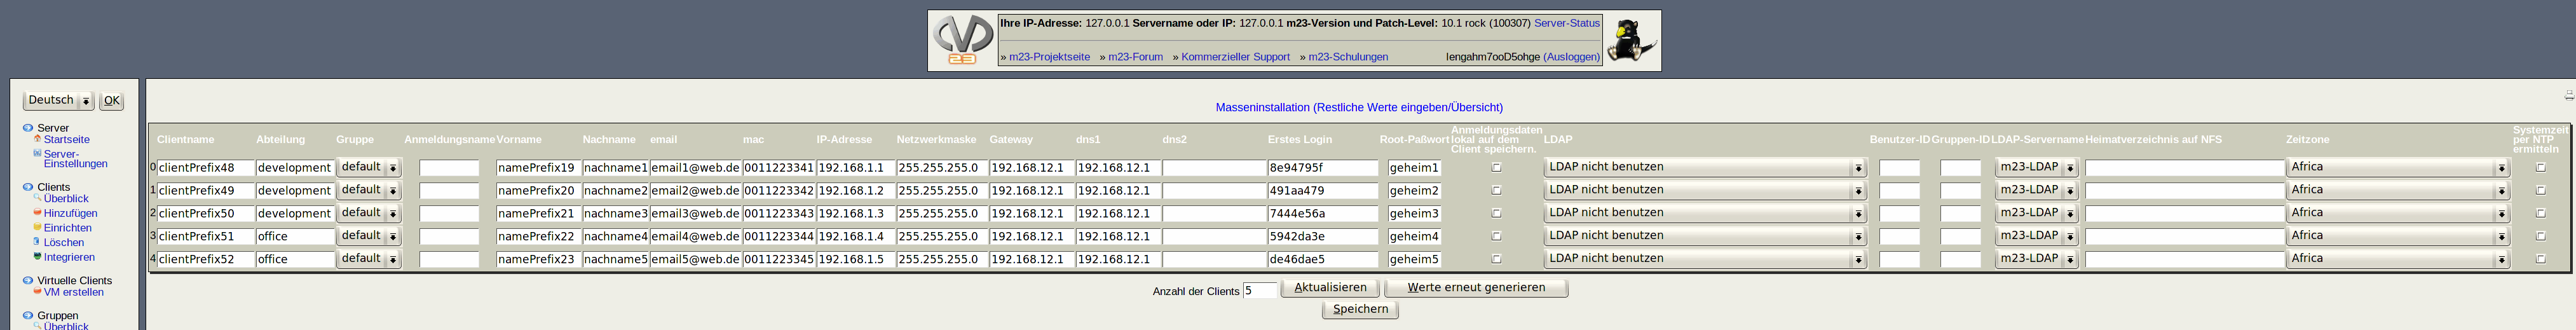
\includegraphics[scale=0.33]{/mdk/doc/manual/screenshots/de/mi_step4.png} \\
\subsection{Anzahl der Clients �ndern}
Sie k�nnen die Anzahl der Clients �ndern, indem Sie bei \textit{"Anzahl der Clients"} die neue Anzahl angeben und danach auf \textit{"Aktualisieren"} klicken, wenn Sie weniger Clients oder auf \textit{"Werte erneut generieren"}, wenn Sie mehr Clients als vorher w�nschen.\\
Werden mehr Clients als zuvor angegeben, so hat dies zur Folge, da� mit einem Klick auf "Werte erneut generieren" die Generatoren die ben�tigten Werte erstellen, bzw. zus�tzliche Werte aus der Datenbank-Datei gelesen werden. Sollten aus der Datenbank-Datei nicht gen�gend Werte ausgelesen werden k�nnen, so m�ssen dieser per Hand in die Tabelle eingegeben werden. Die Generierung von vielen Werten kann u.U. sehr lange dauern, z.B. wenn die IP-Adressen generiert werden sollen und Sie ausgew�hlt haben, da� die IP-Adressen vor Benutzung "angepingt" werden sollen.\\
Klicken Sie abschlie�end auf \textit{"Speichern"}, um die Installation auf den Clients zu starten.\\


\chapter{Tools}
\input{../makeBootDisk.hlp.tex}
\input{../makeBootCD.hlp.tex}

\chapter{m23 license: The GNU General Public License}

\begin{center}
{\parindent 0in

Version 2, June 1991

Copyright \copyright\ 1989, 1991 Free Software Foundation, Inc.

\bigskip

59 Temple Place - Suite 330, Boston, MA  02111-1307, USA

\bigskip

Everyone is permitted to copy and distribute verbatim copies
of this license document, but changing it is not allowed.
}
\end{center}

\begin{center}
{\bf\large Preamble}
\end{center}


The licenses for most software are designed to take away your freedom to
share and change it.  By contrast, the GNU General Public License is
intended to guarantee your freedom to share and change free software---to
make sure the software is free for all its users.  This General Public
License applies to most of the Free Software Foundation's software and to
any other program whose authors commit to using it.  (Some other Free
Software Foundation software is covered by the GNU Library General Public
License instead.)  You can apply it to your programs, too.

When we speak of free software, we are referring to freedom, not price.
Our General Public Licenses are designed to make sure that you have the
freedom to distribute copies of free software (and charge for this service
if you wish), that you receive source code or can get it if you want it,
that you can change the software or use pieces of it in new free programs;
and that you know you can do these things.

To protect your rights, we need to make restrictions that forbid anyone to
deny you these rights or to ask you to surrender the rights.  These
restrictions translate to certain responsibilities for you if you
distribute copies of the software, or if you modify it.

For example, if you distribute copies of such a program, whether gratis or
for a fee, you must give the recipients all the rights that you have.  You
must make sure that they, too, receive or can get the source code.  And
you must show them these terms so they know their rights.

We protect your rights with two steps: (1) copyright the software, and (2)
offer you this license which gives you legal permission to copy,
distribute and/or modify the software.

Also, for each author's protection and ours, we want to make certain that
everyone understands that there is no warranty for this free software.  If
the software is modified by someone else and passed on, we want its
recipients to know that what they have is not the original, so that any
problems introduced by others will not reflect on the original authors'
reputations.

Finally, any free program is threatened constantly by software patents.
We wish to avoid the danger that redistributors of a free program will
individually obtain patent licenses, in effect making the program
proprietary.  To prevent this, we have made it clear that any patent must
be licensed for everyone's free use or not licensed at all.

The precise terms and conditions for copying, distribution and
modification follow.

\begin{center}
{\Large \sc Terms and Conditions For Copying, Distribution and
  Modification}
\end{center}


%\renewcommand{\theenumi}{\alpha{enumi}}
\begin{enumerate}

\addtocounter{enumi}{-1}

\item 

This License applies to any program or other work which contains a notice
placed by the copyright holder saying it may be distributed under the
terms of this General Public License.  The ``Program'', below, refers to
any such program or work, and a ``work based on the Program'' means either
the Program or any derivative work under copyright law: that is to say, a
work containing the Program or a portion of it, either verbatim or with
modifications and/or translated into another language.  (Hereinafter,
translation is included without limitation in the term ``modification''.)
Each licensee is addressed as ``you''.

Activities other than copying, distribution and modification are not
covered by this License; they are outside its scope.  The act of
running the Program is not restricted, and the output from the Program
is covered only if its contents constitute a work based on the
Program (independent of having been made by running the Program).
Whether that is true depends on what the Program does.

\item You may copy and distribute verbatim copies of the Program's source
  code as you receive it, in any medium, provided that you conspicuously
  and appropriately publish on each copy an appropriate copyright notice
  and disclaimer of warranty; keep intact all the notices that refer to
  this License and to the absence of any warranty; and give any other
  recipients of the Program a copy of this License along with the Program.

You may charge a fee for the physical act of transferring a copy, and you
may at your option offer warranty protection in exchange for a fee.

\item

You may modify your copy or copies of the Program or any portion
of it, thus forming a work based on the Program, and copy and
distribute such modifications or work under the terms of Section 1
above, provided that you also meet all of these conditions:

\begin{enumerate}

\item 

You must cause the modified files to carry prominent notices stating that
you changed the files and the date of any change.

\item

You must cause any work that you distribute or publish, that in
whole or in part contains or is derived from the Program or any
part thereof, to be licensed as a whole at no charge to all third
parties under the terms of this License.

\item
If the modified program normally reads commands interactively
when run, you must cause it, when started running for such
interactive use in the most ordinary way, to print or display an
announcement including an appropriate copyright notice and a
notice that there is no warranty (or else, saying that you provide
a warranty) and that users may redistribute the program under
these conditions, and telling the user how to view a copy of this
License.  (Exception: if the Program itself is interactive but
does not normally print such an announcement, your work based on
the Program is not required to print an announcement.)

\end{enumerate}


These requirements apply to the modified work as a whole.  If
identifiable sections of that work are not derived from the Program,
and can be reasonably considered independent and separate works in
themselves, then this License, and its terms, do not apply to those
sections when you distribute them as separate works.  But when you
distribute the same sections as part of a whole which is a work based
on the Program, the distribution of the whole must be on the terms of
this License, whose permissions for other licensees extend to the
entire whole, and thus to each and every part regardless of who wrote it.

Thus, it is not the intent of this section to claim rights or contest
your rights to work written entirely by you; rather, the intent is to
exercise the right to control the distribution of derivative or
collective works based on the Program.

In addition, mere aggregation of another work not based on the Program
with the Program (or with a work based on the Program) on a volume of
a storage or distribution medium does not bring the other work under
the scope of this License.

\item
You may copy and distribute the Program (or a work based on it,
under Section 2) in object code or executable form under the terms of
Sections 1 and 2 above provided that you also do one of the following:

\begin{enumerate}

\item

Accompany it with the complete corresponding machine-readable
source code, which must be distributed under the terms of Sections
1 and 2 above on a medium customarily used for software interchange; or,

\item

Accompany it with a written offer, valid for at least three
years, to give any third party, for a charge no more than your
cost of physically performing source distribution, a complete
machine-readable copy of the corresponding source code, to be
distributed under the terms of Sections 1 and 2 above on a medium
customarily used for software interchange; or,

\item

Accompany it with the information you received as to the offer
to distribute corresponding source code.  (This alternative is
allowed only for noncommercial distribution and only if you
received the program in object code or executable form with such
an offer, in accord with Subsection b above.)

\end{enumerate}


The source code for a work means the preferred form of the work for
making modifications to it.  For an executable work, complete source
code means all the source code for all modules it contains, plus any
associated interface definition files, plus the scripts used to
control compilation and installation of the executable.  However, as a
special exception, the source code distributed need not include
anything that is normally distributed (in either source or binary
form) with the major components (compiler, kernel, and so on) of the
operating system on which the executable runs, unless that component
itself accompanies the executable.

If distribution of executable or object code is made by offering
access to copy from a designated place, then offering equivalent
access to copy the source code from the same place counts as
distribution of the source code, even though third parties are not
compelled to copy the source along with the object code.

\item
You may not copy, modify, sublicense, or distribute the Program
except as expressly provided under this License.  Any attempt
otherwise to copy, modify, sublicense or distribute the Program is
void, and will automatically terminate your rights under this License.
However, parties who have received copies, or rights, from you under
this License will not have their licenses terminated so long as such
parties remain in full compliance.

\item
You are not required to accept this License, since you have not
signed it.  However, nothing else grants you permission to modify or
distribute the Program or its derivative works.  These actions are
prohibited by law if you do not accept this License.  Therefore, by
modifying or distributing the Program (or any work based on the
Program), you indicate your acceptance of this License to do so, and
all its terms and conditions for copying, distributing or modifying
the Program or works based on it.

\item
Each time you redistribute the Program (or any work based on the
Program), the recipient automatically receives a license from the
original licensor to copy, distribute or modify the Program subject to
these terms and conditions.  You may not impose any further
restrictions on the recipients' exercise of the rights granted herein.
You are not responsible for enforcing compliance by third parties to
this License.

\item
If, as a consequence of a court judgment or allegation of patent
infringement or for any other reason (not limited to patent issues),
conditions are imposed on you (whether by court order, agreement or
otherwise) that contradict the conditions of this License, they do not
excuse you from the conditions of this License.  If you cannot
distribute so as to satisfy simultaneously your obligations under this
License and any other pertinent obligations, then as a consequence you
may not distribute the Program at all.  For example, if a patent
license would not permit royalty-free redistribution of the Program by
all those who receive copies directly or indirectly through you, then
the only way you could satisfy both it and this License would be to
refrain entirely from distribution of the Program.

If any portion of this section is held invalid or unenforceable under
any particular circumstance, the balance of the section is intended to
apply and the section as a whole is intended to apply in other
circumstances.

It is not the purpose of this section to induce you to infringe any
patents or other property right claims or to contest validity of any
such claims; this section has the sole purpose of protecting the
integrity of the free software distribution system, which is
implemented by public license practices.  Many people have made
generous contributions to the wide range of software distributed
through that system in reliance on consistent application of that
system; it is up to the author/donor to decide if he or she is willing
to distribute software through any other system and a licensee cannot
impose that choice.

This section is intended to make thoroughly clear what is believed to
be a consequence of the rest of this License.

\item
If the distribution and/or use of the Program is restricted in
certain countries either by patents or by copyrighted interfaces, the
original copyright holder who places the Program under this License
may add an explicit geographical distribution limitation excluding
those countries, so that distribution is permitted only in or among
countries not thus excluded.  In such case, this License incorporates
the limitation as if written in the body of this License.

\item
The Free Software Foundation may publish revised and/or new versions
of the General Public License from time to time.  Such new versions will
be similar in spirit to the present version, but may differ in detail to
address new problems or concerns.

Each version is given a distinguishing version number.  If the Program
specifies a version number of this License which applies to it and ``any
later version'', you have the option of following the terms and conditions
either of that version or of any later version published by the Free
Software Foundation.  If the Program does not specify a version number of
this License, you may choose any version ever published by the Free Software
Foundation.

\item
If you wish to incorporate parts of the Program into other free
programs whose distribution conditions are different, write to the author
to ask for permission.  For software which is copyrighted by the Free
Software Foundation, write to the Free Software Foundation; we sometimes
make exceptions for this.  Our decision will be guided by the two goals
of preserving the free status of all derivatives of our free software and
of promoting the sharing and reuse of software generally.

\begin{center}
{\Large\sc
No Warranty
}
\end{center}

\item
{\sc Because the program is licensed free of charge, there is no warranty
for the program, to the extent permitted by applicable law.  Except when
otherwise stated in writing the copyright holders and/or other parties
provide the program ``as is'' without warranty of any kind, either expressed
or implied, including, but not limited to, the implied warranties of
merchantability and fitness for a particular purpose.  The entire risk as
to the quality and performance of the program is with you.  Should the
program prove defective, you assume the cost of all necessary servicing,
repair or correction.}

\item
{\sc In no event unless required by applicable law or agreed to in writing
will any copyright holder, or any other party who may modify and/or
redistribute the program as permitted above, be liable to you for damages,
including any general, special, incidental or consequential damages arising
out of the use or inability to use the program (including but not limited
to loss of data or data being rendered inaccurate or losses sustained by
you or third parties or a failure of the program to operate with any other
programs), even if such holder or other party has been advised of the
possibility of such damages.}

\end{enumerate}


\begin{center}
{\Large\sc End of Terms and Conditions}
\end{center}


\pagebreak[2]

\section*{Appendix: How to Apply These Terms to Your New Programs}

If you develop a new program, and you want it to be of the greatest
possible use to the public, the best way to achieve this is to make it
free software which everyone can redistribute and change under these
terms.

  To do so, attach the following notices to the program.  It is safest to
  attach them to the start of each source file to most effectively convey
  the exclusion of warranty; and each file should have at least the
  ``copyright'' line and a pointer to where the full notice is found.

\begin{quote}
one line to give the program's name and a brief idea of what it does. \\
Copyright (C) yyyy  name of author \\

This program is free software; you can redistribute it and/or modify
it under the terms of the GNU General Public License as published by
the Free Software Foundation; either version 2 of the License, or
(at your option) any later version.

This program is distributed in the hope that it will be useful,
but WITHOUT ANY WARRANTY; without even the implied warranty of
MERCHANTABILITY or FITNESS FOR A PARTICULAR PURPOSE.  See the
GNU General Public License for more details.

You should have received a copy of the GNU General Public License
along with this program; if not, write to the Free Software
Foundation, Inc., 59 Temple Place - Suite 330, Boston, MA  02111-1307, USA.
\end{quote}

Also add information on how to contact you by electronic and paper mail.

If the program is interactive, make it output a short notice like this
when it starts in an interactive mode:

\begin{quote}
Gnomovision version 69, Copyright (C) yyyy  name of author \\
Gnomovision comes with ABSOLUTELY NO WARRANTY; for details type `show w'. \\
This is free software, and you are welcome to redistribute it
under certain conditions; type `show c' for details.
\end{quote}


The hypothetical commands {\tt show w} and {\tt show c} should show the
appropriate parts of the General Public License.  Of course, the commands
you use may be called something other than {\tt show w} and {\tt show c};
they could even be mouse-clicks or menu items---whatever suits your
program.

You should also get your employer (if you work as a programmer) or your
school, if any, to sign a ``copyright disclaimer'' for the program, if
necessary.  Here is a sample; alter the names:

\begin{quote}
Yoyodyne, Inc., hereby disclaims all copyright interest in the program \\
`Gnomovision' (which makes passes at compilers) written by James Hacker. \\

signature of Ty Coon, 1 April 1989 \\
Ty Coon, President of Vice
\end{quote}


This General Public License does not permit incorporating your program
into proprietary programs.  If your program is a subroutine library, you
may consider it more useful to permit linking proprietary applications
with the library.  If this is what you want to do, use the GNU Library
General Public License instead of this License.


\end{document}
